% REMEMBER: You must not plagiarise anything in your report. Be extremely careful.

\documentclass{l4proj}
\usepackage{pdfpages}
\usepackage{float}
\usepackage[table,svgnames,table,xcdraw]{xcolor}
\usepackage[colorinlistoftodos]{todonotes}
\usepackage{svg}
\usepackage{amsmath}
\usepackage{graphicx}
    
%
% put any additional packages here
%

\begin{document}

%==============================================================================
%% METADATA
\title{Probabilistic Nomograms}
\author{Barkin Bryce}
\date{March 22, 2024}

\maketitle

%==============================================================================
%% ABSTRACT
\begin{abstract}
    Studies suggest that people face various difficulties when making probabilistic calculations due to their lack of practical experience and technical background, beginning in school. 
    Nomograms, also known as alignment charts, are graphs where multiple axis represent the values of variables in a given equation, with an another axis that includes the solution space that is found by connecting a straight line between the axis. They can provoke interest as they are not well known, and can be a useful tool in performing probabilistic calculations. 
    In this project, a program was developed to allow people to create probabilistic relationships in any equation by creating a probabilistic nomogram that can be used in educational and professional settings. There was a focus on creating a digital version of any existing paper based nomogram, and probabilistic distributions could be included easily afterwards. 

    This program was evaluated to show that it can work correctly after users understand the flow of the application, and participants stated that they would be interested in using it many fields. Addressing the difficulties faced by participants when building a digital nomogram would be the main focus of any future work on this topic. 
\end{abstract}

%==============================================================================

% EDUCATION REUSE CONSENT FORM
% If you consent to your project being shown to future students for educational purposes
% then insert your name and the date below to  sign the education use form that appears in the front of the document. 
% You must explicitly give consent if you wish to do so.
% If you sign, your project may be included in the Hall of Fame if it scores particularly highly.
%
%Please note that you are under no obligation to sign 
%this declaration, but doing so would help future students.
%
\def\consentname {Barkin Bryce} % your full name
\def\consentdate {20th January 2024} % the date you agree
%
\educationalconsent


%==============================================================================
\tableofcontents

%==============================================================================
%% Notes on formatting
%==============================================================================
% The first page, abstract and table of contents are numbered using Roman numerals and are not
% included in the page count. 
%
% From now on pages are numbered
% using Arabic numerals. Therefore, immediately after the first call to \chapter we need the call
% \pagenumbering{arabic} and this should be called once only in the document. 
%
% Do not alter the bibliography style.
%
% The first Chapter should then be on page 1. You are allowed 40 pages for a 40 credit project and 30 pages for a 
% 20 credit report. This includes everything numbered in Arabic numerals (excluding front matter) up
% to but excluding the appendices and bibliography.
%
% You must not alter text size (it is currently 10pt) or alter margins or spacing.
%
%
%==================================================================================================================================
%
% IMPORTANT
% The chapter headings here are **suggestions**. You don't have to follow this model if
% it doesn't fit your project. Every project should have an introduction and conclusion,
% however. 
%
%==================================================================================================================================
\chapter{Introduction}\label{introduction}

% reset page numbering. Don't remove this!
\pagenumbering{arabic} \label{intro}

\section{Motivation}
Before the invention of scientific calculators and computers, nomograms were used to quickly calculate the value of a missing value in a mathematical formula. 

Nomograms, also known as alignment charts, are graphical instruments designed to calculate the value of a missing parameter in a mathematical calculation by extending a thread or straightedge along a graph to find the point of interception with the axes of the missing variable. 

\begin{figure}[hbt!]
    
    \centering
    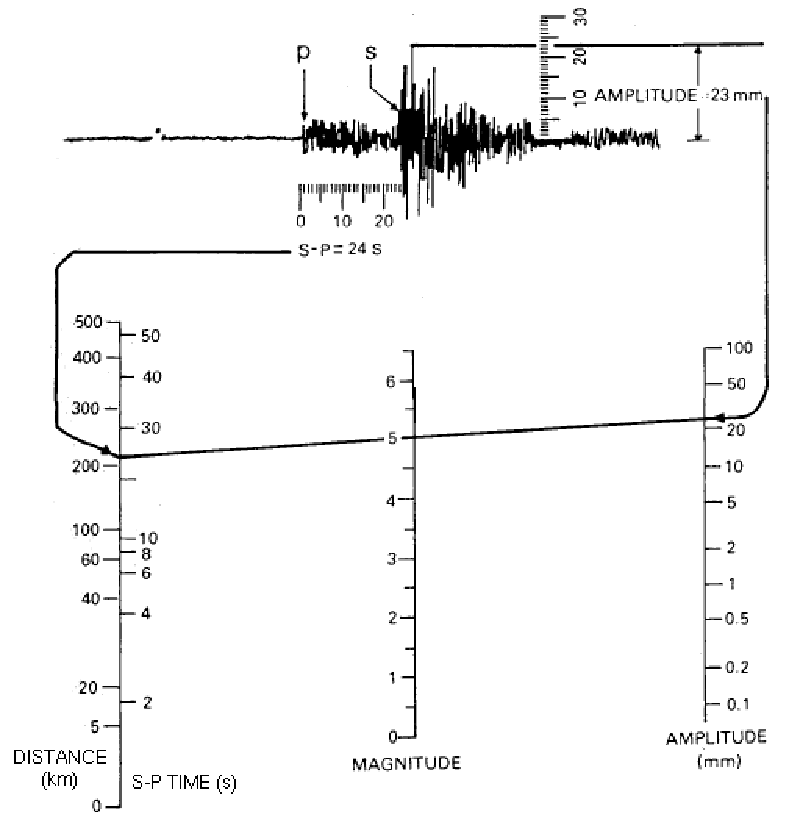
\includegraphics[width=.75\linewidth]{dissertation/images/myFigures/introduction/richter-scale.pdf}    

    \caption{
    A nomogram that comprises the distance of seismic waves in an earthquake from its origin and its amplitude with the corresponding Richter magnitude in the middle. \protect \citep{stimac_what_nodate}}

    % use the notation fig:name to cross reference a figure
    \label{fig:richter} 
\end{figure}

In most cases, the user knows the value of most of the variables, and they can directly calculate the value of the missing value. Suppose the values of multiple variables are unknown. In that case, a person can move a ruler around on the nomogram and see how the change in one or multiple variables can impact another. The ease of use of nomograms allows students, doctors, engineers, scientists and others to calculate a value in a practical environment, such as in medicine, made popular due to the blood physiology nomograms made by L. J. Henderson \citep{hankins_blood_1999}, construction, defence and more. Even in the age of modern portable computers, nomograms offer various advantages. They do not require power, access to the Internet, or long documentation on how to operate it. The fixed ranges of the axis of nomograms provide a built-in fail-safe mechanism against incorrect inputs by limiting the values of the variables to realistic ranges, which allows people who are not experts in the field to ensure that they have followed the respective methods correctly.     

As opposed to calculations with variables with fixed values, there can also be scenarios where a variable is described by a probability distribution, creating uncertainty. Other variables cannot be calculated accurately from the variable given by a probability distribution due to the high inaccuracy caused by the nature of probability distributions. In addition to the impact of the probability distribution, as many nomograms are used to calculate nonlinear mathematical relationships, a slight change in one variable can severely impact another due to the impacts of compounding uncertainties.  

Therefore, the range of values that the missing parameter can take, the combination of a nonlinear relationship in a mathematical equation, and a large range of values can easily exceed the estimation of the average person and alter their approach to a problem.  

For example, imagine a nutritionist who is working on a body mass index nomogram and wants to use a normal distribution to represent the height of the population to see the correlation between a specific body mass index and a weight to the probability of them being of a certain height to visually interpret the relationship between the height of a population against a BMI and weight. Incorporating probability distributions into a classical nomogram would be quite time-consuming, as it would be incredibly challenging to accurately physically draw a probability distribution on a paper-based nomogram and align it with precision. Another example is understanding the probabilistic relationship between different factors in risk assessment, which can help identify potential outcomes and assess their likelihood, enabling better risk mitigation strategies. Similarly, in decision-making processes involving complex systems or multiple variables, considering the uncertainty inherent in each variable allows for more robust and realistic analyses.
Understanding the impact of a probability distribution when calculating another variable is essential for various fields and professions. In many real-world scenarios, data is inherently uncertain, and probability distributions rather than fixed values describe variables. For instance, in finance, stock prices are often modelled using stochastic processes, leading to uncertainty in future prices. In epidemiology, the spread of diseases may follow probabilistic patterns influenced by factors such as population density, immunity levels, and transmission rates.

Professionals can better account for uncertainty and make more informed decisions by incorporating probability distributions into calculations. 

Furthermore, recognizing the impact of probability distributions on calculations helps individuals interpret results accurately. Instead of relying solely on point estimates, which may overlook the variability and uncertainty present in the data, professionals can use probabilistic models to generate a range of possible outcomes and their associated probabilities. This probabilistic approach fosters a deeper understanding of the inherent uncertainties in the studied system and promotes more cautious and nuanced interpretations of results.

Building a nomogram to represent probabilistic relationships using a computer can save time, be easier to use than a paper-based nomogram with probabilistic relationships, provide a wide range of customizability and accessibility features, and deliver visual interactions that provide a more accurate reading. This approach would combine the advantages of a paper-based nomogram with the quality-of-life improvements brought by modern computers. 
\section{Aim}
This project aims to develop a tool for creating and viewing probabilistic nomograms and providing visual interactions to the user. 

The overall goal of this program is to allow users to build probabilistic nomograms where they can use a probability distribution to represent the values of a chosen variable in any computer-recognised format and be able to interact with the nomogram by moving a digital ruler, referred to as the \textit{isopleth} in nomography. The user should not be required to know how to build a nomogram from an equation; rather, they should be able to use any nomogram they find and use their own measurements or measurements from third parties to be able to make predictions on a variable, be able to save their datasets, probability distributions and any other relevant information as they wish. 

\section{Report Structure} 
In this chapter, the motivation and aim behind the development of probabilistic nomograms were outlined to clarify the application's overall objective and how it aims to contribute to the science of nomography. The remainder of this paper will discuss how the motivation for Probabilistic Nomograms was developed into a working application and how the aims were met. The structure of this report is as follows:
\begin{itemize}
    \item \Cref{background} gives a more detailed description of nomograms, their educational benefits and how they are constructed, discusses existing applications that produce nomograms and outlines their advantages and limitations.
    \item \Cref{requirements} outlines the requirements specification formulated from user stories to develop a complete set of functional and non-functional requirements.
    \item \Cref{design} discusses the application's design process, tools and technologies picked to develop the application, explaining the rationale behind the user interface design and linking the choices to the functional and non-functional requirements outlined in the requirements specification. 
    \item \Cref{implementation} explains the application implementation and the software development strategies.
    \item \Cref{evaluation} covers the evaluation strategy, including monitored user testing, performance evaluation, and requirement validation. 
    \item \Cref{conclusion} summarises the report, discusses potential future enhancements and reflects on the project. 
    
\end{itemize}



%==================================================================================================================================
\chapter{Background}\label{background}


Nomograms can be classified into several types, depending on the mathematical functions used in the general equation. 
The nomogram formulas range from functions related to the simple addition of variables to relationships represented as matrices. \citep{boulet_PyNomo_2023} 

    \section{The Geometry of Nomograms}


Nomograms composed of straight scales can be designed by analyzing their geometric properties, leading to the construction of various interesting nomograms. 
\begin{figure}[H]
    \centering
    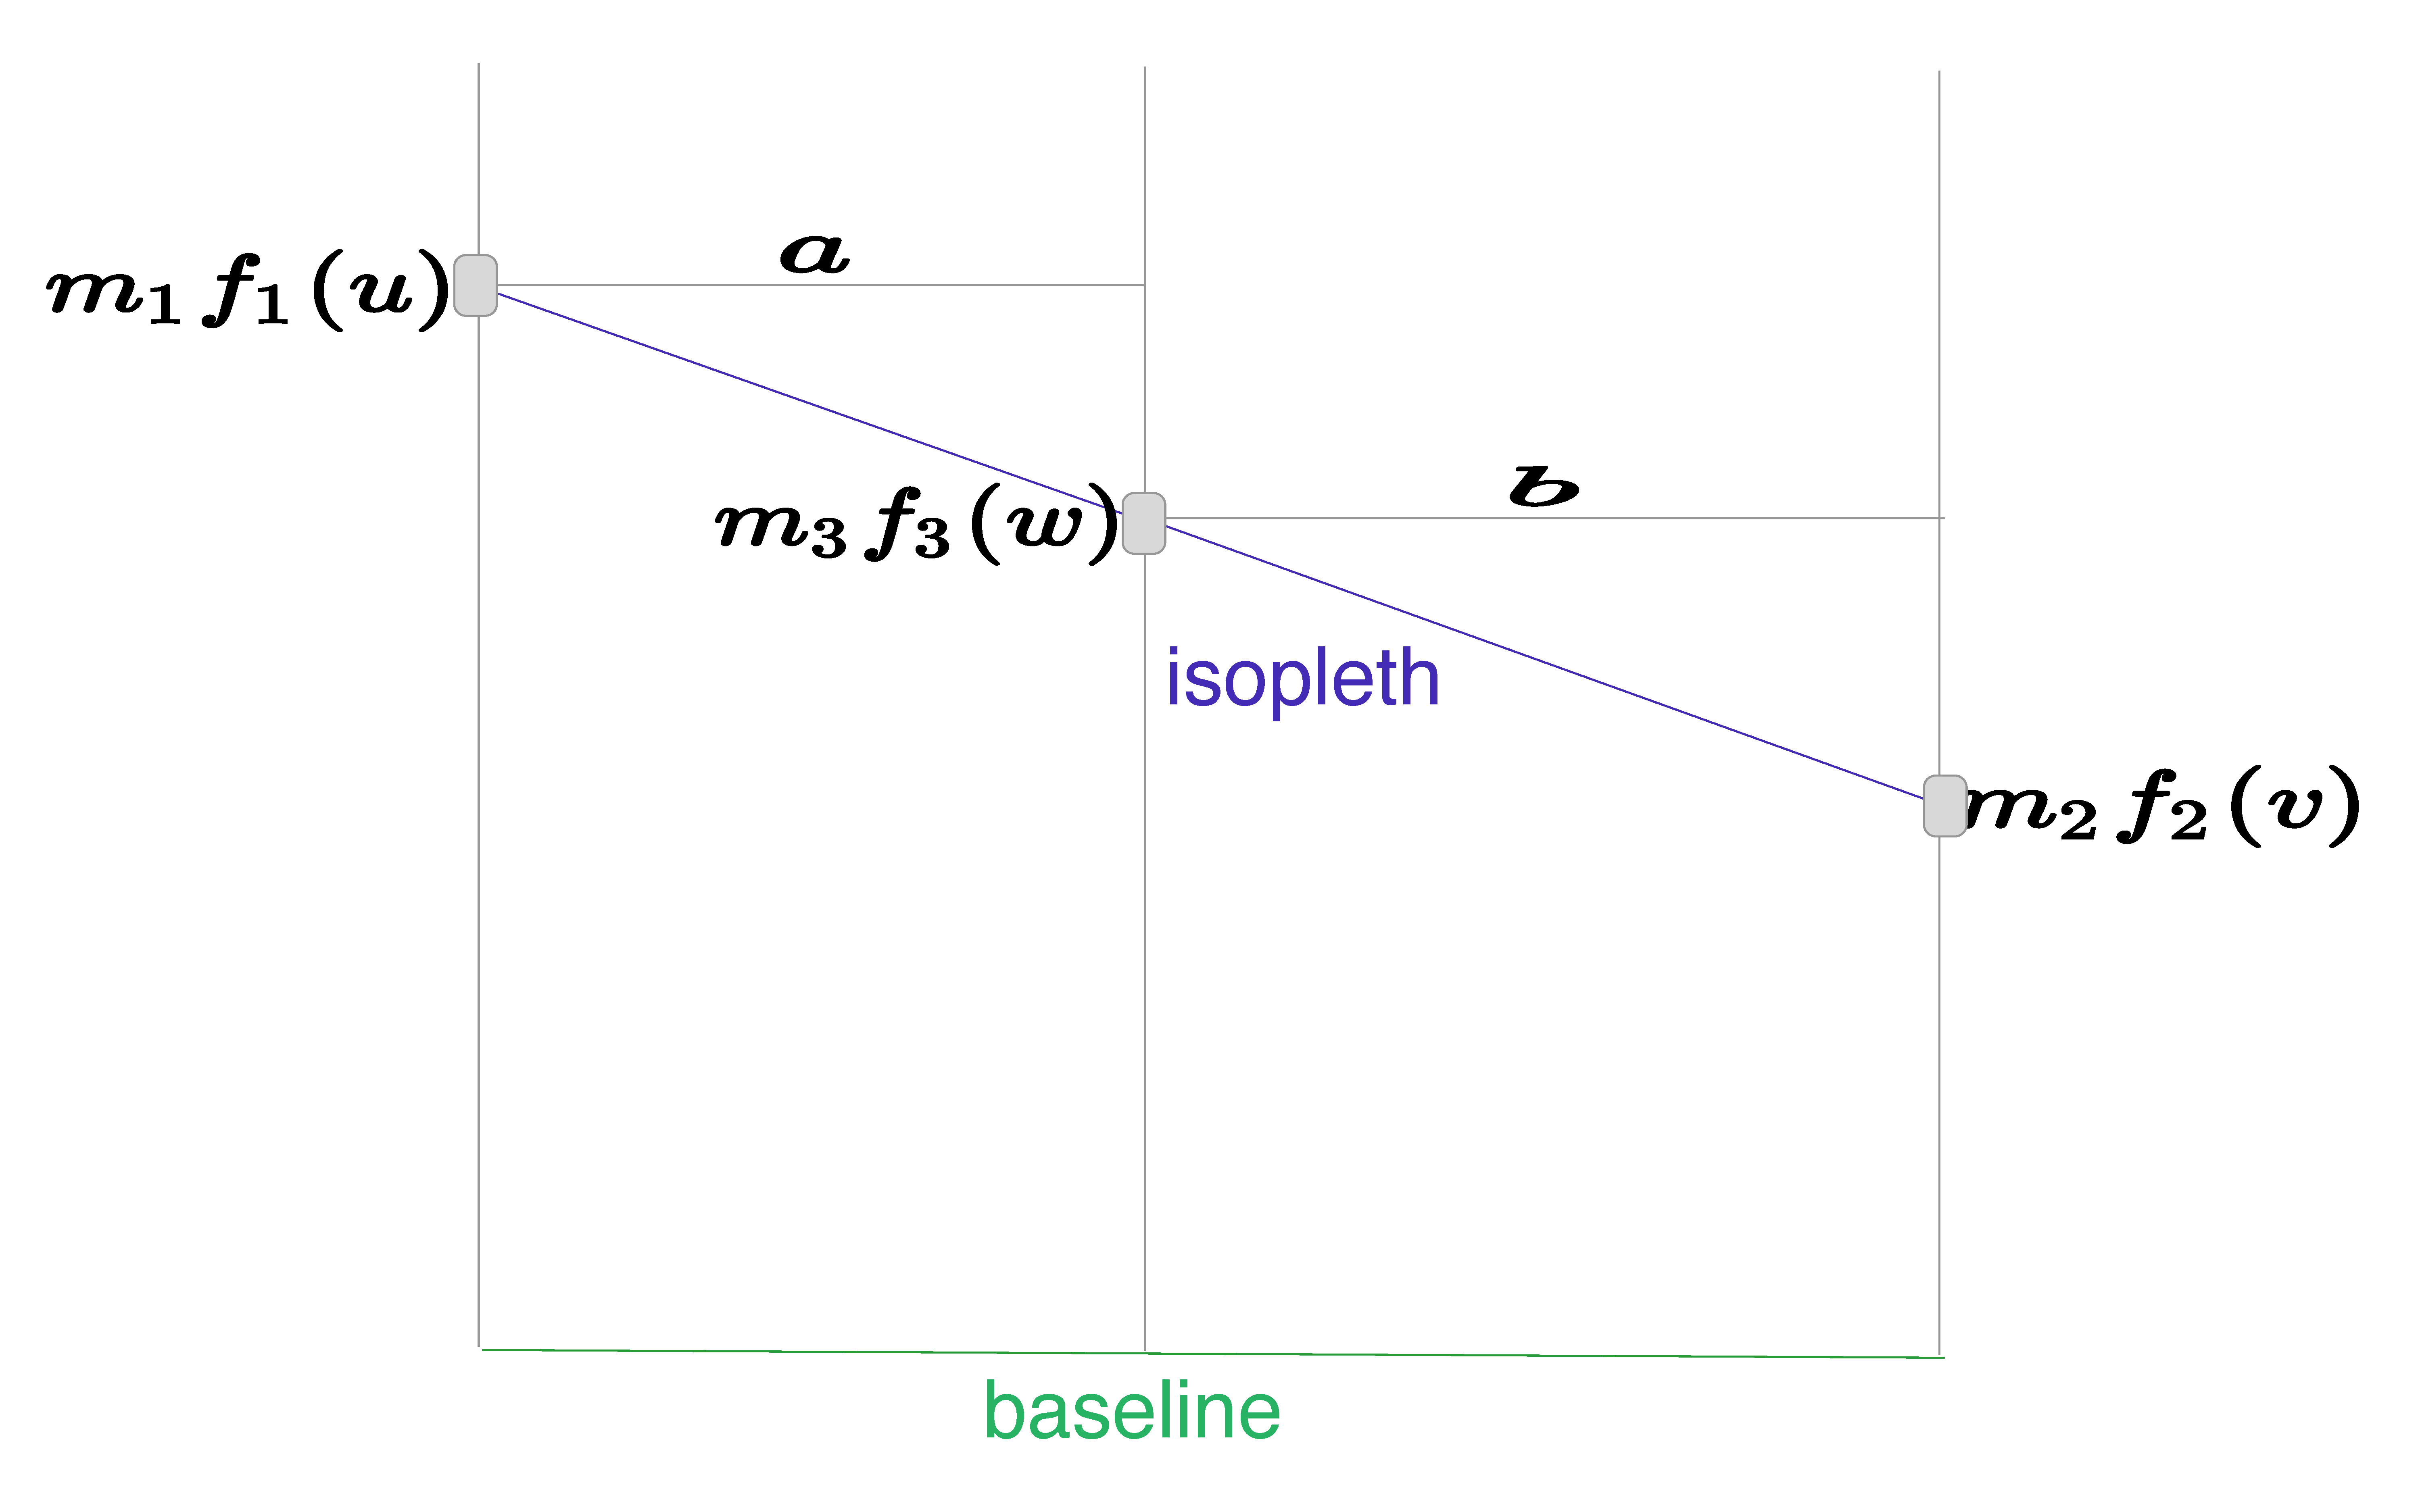
\includegraphics[width=0.75\linewidth]{dissertation/images/myFigures/background/nomogram.pdf}
    \caption{A simple parallel nomogram}
    \label{fig:nomogram}
\end{figure}

 \Cref{fig:nomogram} illustrates the basic parallel scale nomogram for calculating a value $f_3(w)$ as the sum of two functions $f_1(u)$ and $f_2(v)$:

\[ f_1(u) + f_2(v) = f_3(w) \]

Each function is plotted vertically using a corresponding scaling factor $m_1$, $m_2$ and $m_3$ that provides a conveniently sized nomogram. The spacing of the lines is represented as $a$ and $b$. By similar triangles, 

\[ \frac{m_1f_1(u) - m_3f_3(w)}{a} = \frac{m_3f_3(w) - m_2f_2(v)}{b} \]

This can be rearranged as:

\[ m_1f_1(u) + \left(\frac{a}{b}\right)m_2f_2(v) = \left(1 + \frac{a}{b}\right)m_3f_3(w) \]

To arrive at the original equation $f_1(u) + f_2(v) = f_3(w)$, all terms involving $m$, $a$, and $b$ are canceled out, which is achieved by setting $m_1 = \frac{a}{b} m_2 = \left(1 + \frac{a}{b}\right) m_3$. The left half of this relationship provides the relative scaling of the two outer scales, and the outer parts provide the scaling of the middle scale:

\[ \frac{m_1}{m_2} = \frac{a}{b}, \quad m_3 = \frac{m_1m_2}{m_1+ m_2} \]

For the case where the middle scale is located halfway between the outer scales, $a = b$, and in this case, $m_1 = m_2$ and $m_3 = \frac{1}{2}m_1$.

Using logarithmic scales expands parallel scale nomograms to very complicated equations. Logarithms allow multiplications to be represented by additions and powers to be represented by multiplications.

For example, if we have an equation such as $f_1(u) \cdot f_2(v) = f_3(w)$, we can replace it with:

\[ \log[f_1(u) \cdot f_2(v)] = \log f_3(w) \]

or

\[ \log f_1(u) + \log f_2(v) = \log f_3(w) \]

This conversion simplifies the equation, and we can plot these logs on the scales without solving symbolically for the variable.

Let's create a nomogram for the engineering equation $(u + 0.64)^{0.58}(0.74v) = w$. Assuming engineering ranges $1.0 < u < 3.5$ and $1.0 < v < 2.0$:

\[ 0.58 \log(u + 0.64) + \log(0.74v) = \log w \]
\[ 0.58 \log(u + 0.64) + \log v = \log w - \log(0.74) \]

We will directly plot the three components as our $u$, $v$, and $w$ scales. The scaling factors are calculated by dividing the final desired height of the $u$ and $v$ scales by the ranges of $u$ and $v$. Let's denote the desired height of the scales as 6 inches and set the width of the chart to 3 inches:

\[ m_1 = \frac{6}{0.58 \log(3.5 + 0.64) - 0.58 \log(1 + 0.64)} \]
\[ m_2 = \frac{6}{\log 2.0 - \log 1.0} \]
\[ m_3 = \frac{m_1 m_2}{m_1 + m_2} \]

\[ \frac{a}{b} = \frac{m_1}{m_2}, \quad a + b = 3 \]

Solving for $a$ and $b$, we can then draw the scales accordingly. \citep{doerfler_art_2008}

Nomograms like the "N Chart" or "Z Chart" are named for their shape, resembling the letter "Z." These charts can be used to solve equations involving division. The slanting middle scale can be adjusted to accommodate different problem requirements.

\begin{itemize}
    \item Proportional charts solve equations with four unknowns of the type $\frac{f_1(u)}{f_2(v)} = \frac{f_3(w)}{f_4(t)}$. These charts utilize scaling factors for the outer scales to ensure proportional relationships between variables.
    \item Concurrent charts solve equations of the type $\frac{1}{f_1(u)} + \frac{1}{f_2(v)} = \frac{1}{f_3(w)}$, such as the effective resistance of two parallel resistors.
    \item Four-variable charts combine two separate charts of any type to solve a four-variable equation with one unknown.
    \item Curved scale charts involve curved scales and are designed using determinants, offering a more straightforward approach to designing nomograms with curved scales.
\end{itemize}
The various types of nomograms provide accurate graphical methods for solving equations across different domains, offering flexibility and simplicity in their application. The variability of nomogram types leads to a nomogram that looks like an alignment chart of three parallel axes to alignment charts where the axes are perpendicular to each other. The axes can have linear, logarithmic, trigonometric, and exponential shapes and scales. 

Some computer programs can construct nomograms without defining probabilistic relationships, such as PyNomo, described in \Cref{PyNomo}, where a user defines multiple \textit{blocks} of axes, their ranges and the scaling of values on the axis, the general \textit{type}, and a nomogram in \LaTeX\ format is produced through a series of calculations. 

We can produce a probabilistic nomogram through the following steps:
\begin{enumerate}
    \item First, a general nomogram will be designed where the values of the variables are initially fixed. 
    \item The nomogram can be transformed into a probabilistic nomogram by replacing a fixed value point with a probabilistic relationship, such as a normal distribution, displayed as a box and whisker plot, as a series of points with varying radii depending on their respective probability, as a curve, or through other types of graph visualisations. 
\end{enumerate}

The intersection of these distributions can identify the probability density or the probability mass value and the standard deviation at a specific point, providing insights into the possible values the missing variables can take. The user can then interpret the results following the rules of the subject area to which the nomogram relates and the probabilistic distribution and methods used.   

\section{Challenges Faced by Students in Solving Probabilistic Problems}
Students' challenges in understanding probabilistic computations are multifaceted and have significant implications for their learning outcomes. Despite probability theory's crucial role in everyday life and various disciplines, students often encounter difficulties grasping its concepts and applying them effectively in problem-solving scenarios. \citep{arum_students_2018}

One prominent issue lies in students' conceptual understanding. They may struggle to comprehend the fundamental concepts underlying probability theory, such as the principles of randomness, independence, and conditional probability. These conceptual errors hinder their ability to interpret problem scenarios accurately and formulate appropriate strategies for solving them. Additionally, students may fail to appreciate the relationships between different variables or events within a probabilistic context, further impeding their problem-solving skills.

Procedural errors also pose significant challenges for students. Even if they have a basic understanding of probability concepts, they may falter in correctly applying the relevant formulas or algorithms. This could stem from a lack of practice, inadequate familiarity with mathematical manipulations, or misconceptions about the procedural steps involved in solving probabilistic problems.

Technical errors, including mathematical content knowledge deficits or carelessness, further compound students' difficulties. These errors may arise from gaps in understanding related mathematical topics or inaccuracies in computations. Carelessness, such as overlooking critical details or making calculation mistakes, can lead to incorrect solutions despite the requisite knowledge and skills.

Moreover, probabilistic problem-solving demands a synthesis of procedural, conceptual, and real-world knowledge. Students must understand abstract mathematical concepts and apply them in practical contexts to analyze and make informed decisions about uncertain events or outcomes. Integrating knowledge domains can be particularly challenging for students, especially if they struggle to bridge the gap between theoretical concepts and their real-world implications.

\section{Benefits of Interactive Nomograms in the 21st Century}


The potential benefits of nomograms for modern use are best described in \citep{martinez-pagan_nomography_2022}:

"...In this way, the actual importance of including nomography as a
valuable computational tool in an academic context, such as sciences and
engineering studies, could be justified by the next points: 
\begin{enumerate}
    \item it can be attractive and provoke interest, potentially because nomograms are unusual, 
    \item it might provide the basic skills to design and interpret nomograms, avoiding that this centenary knowledge might become utterly extinct from universities, 
    \item  it would contribute to a better understanding of complex formulas and how are associated with their variables, as well as the sensitivity of the results to changes in those variables, 
    \item it may help those people who prefer pictures to equations understand the inputs and results of complex calculations, 
    \item  it could benefit from modern computing, such as open-source codes and more advanced design assistance software to produce in seconds outstanding and customized nomograms, which could be useful and reliable for repetitive tasks, and
    \item it could solve accurately and quickly struggling situations where the
    access to computers or handheld calculators might not be available. "
\end{enumerate}

Interactive nomograms are an easy-to-use and intuitive way of visualising complex relationships between multiple variables. They allow users to interact with the graphical representation, making understanding how different variables impact the outcome easier. Unlike traditional nomograms, interactive ones enable users to manipulate variables in real-time and see the values of the variables more precisely. 

Interactive nomograms can also benefit by sharing the advantage that regular nomograms have, through kinesics, to manipulate data rather than simply reading tables or graphs. \citep{schwartz_physical_1999}

One of the significant technological developments since the invention of nomography is the quick development of new statistical and data analytics models. Real-time data collection and sharing are becoming more prevalent through platforms such as the Office for National Statistics website, where statistical models relating to almost every natural phenomenon can be found. Incorporating these benefits together can improve students' understanding of probabilistic computations. 


\section{Existing Products}

Several applications let users build nomograms with probabilistic distributions. These apps are built using R, Stata, SAS or Orange. However, these applications build nomograms from logistic regressions and Bayesian analysis of datasets provided by users rather than using a mathematical formula to produce a nomogram and replace the fixed points with probabilistic distributions. Examples include DynNom, simpleNomo, and the nomogram builder in Orange. \citep{hutchison_nomograms_2004} As this project aims to create a program that uses nomograms that represent mathematical relationships rather than logistic regressions between variables in existing datasets, we will not discuss them further. 


\subsection{PyNomo} \label{PyNomo}

As mentioned, PyNomo is an open-source Python library built to build nomograms. 

\subsubsection{{Advantages}}

\begin{itemize}
    \item PyNomo is highly customisable, allowing users to draw any chosen nomogram of the predefined types.  
    \item Nomographs can be merged. 
    \item Nomograms can be drawn with high accuracy and precision, with the user able to select the tick levels of the axis. 
\end{itemize}

\subsubsection{{Limitations}}

\begin{itemize}
    \item PyNomo does not support user interaction, as nomograms can only be used in their classical way by extending a straight line along the axis. 
    \item PyNomo axes have fixed values, which means that probabilistic relationships cannot be visualised. 
    \item There is a learning curve to building nomograms with PyNomo as the user has to determine the 'type' of the nomogram, specify all the characteristics of the nomogram, and create a JSON file, which is time-consuming for people who want to add a probabilistic relationship to an existing nomogram.  

    While PyNomo is an excellent application overall, it does not have the features specified in our application goals. 

    
\end{itemize}


\subsection{Janomo}

Janomo is a Java application that lets users handpick an axis from a Nomogram by drawing lines and curves on an existing nomogram and visualising it. 

\begin{figure} [H]
    \centering
    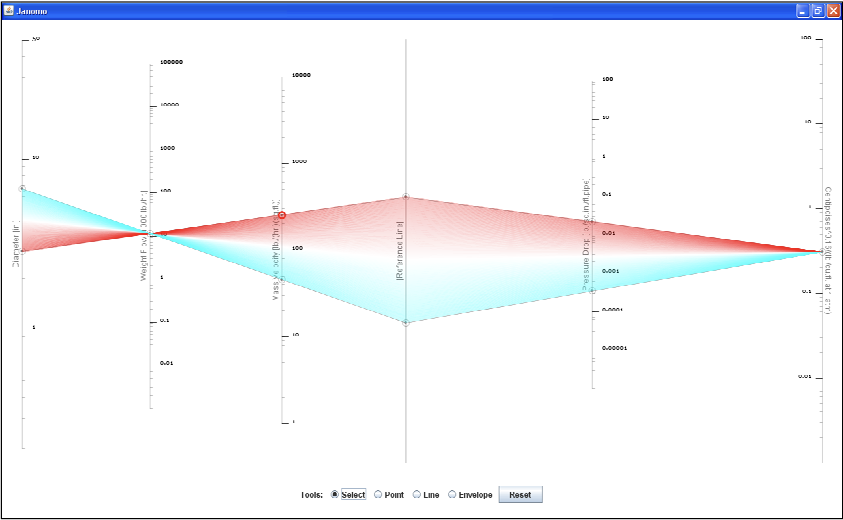
\includegraphics[width=.8\linewidth]{dissertation/images/myFigures/background/janomo.png}
    \caption{A screenshot of Janomo, an interactive nomogram rendering application built in Java, displaying the nomogram for pipe flow turbulence, as originally built by Generaux. \citep{howison_constructing_nodate}}
    \label{fig:janomo}
\end{figure} 

\subsubsection{{Advantages}}
\begin{itemize}
    \item The application allows users to use any chosen nomogram and draw parallel, sloped, and turning axes. They can also see the exact value of the nomograms. 
    \item Users can draw envelopes to visualise how a range along one axis changes across the nomogram, given two fixed points.

\end{itemize}
\subsubsection{{Limitations}}
\begin{itemize}
    \item There is no feature to add or interact with probability distributions.
    
    \item Manually selecting the axis positions leads to inaccuracies with the calculations. 
    \item The program is no longer distributed, and no executable programs were found. 
    
\end{itemize}

\subsection{Newmograms}

Newmograms is a web application that allows users to interact with nomograms built using PyNomo. 

\subsubsection{{Advantages}}
\begin{itemize}
    \item Users can interact with a nomogram and see the exact value on the axis. 
    \item The application allows users to lock the movement of a slider on an axis, which allows users to have effective control over the application. 
\end{itemize}

\subsubsection{{Limitations}}

\begin{itemize}

    \item Only three axes can be shown on a nomogram.
    \item Newmograms rely on a script similar to PyNomo, which means that probabilistic distributions cannot be visualised.
    \item The application uses points generated from PyNomo, which limits user freedom when interacting. 
    \item There is also a slight learning curve for the application, as users have to predefine the nomograms. 
    
    
\end{itemize}

%==================================================================================================================================
\chapter{Analysis/Requirements}\label{requirements}
A list of feature requirements was discussed in weekly meetings with Dr. John Williamson, this project's supervisor. 

The program's requirements evolved as research into the existing nomogram applications, statistical software, and literature was conducted. 

\section{Problem Specification}

The expectations from the program are as stated below. 
The main goal of this project was to provide users with an interactive tool to perform calculations in any subject area where the values needed to perform calculations are not fixed and instead represented by a probability distribution. It was hypothesised that this could be achieved by allowing users to import a nomogram of their choosing, determine and input a probability distribution for an unknown variable and be able to interact with the unknown variable to formulate an understanding of how other variables react to the change in the probabilistic distribution. The usability of this program and hypothesis will be tested through user testing and evaluation.
The functional requirements define the actions users should be able to perform, and the non-functional requirements are the program's requirements.  
\subsection{User stories}
Three user scenarios were developed to describe how users from different backgrounds might interact with the system. 

\begin{itemize}
    \item Mike uses a nomogram with probabilistic distributions that combine factors like genetic predisposition, lifestyle choices, and environmental exposure to estimate the patient's risk of developing cancer. This nomogram visually represents the patient's risk and helps the doctor determine the appropriate screening and prevention strategies.
    \item Helen is working with a client with a unique financial profile, including income, credit score, and debt-to-income ratio.
    Based on these factors, Helen would use a nomogram with probabilistic distributions to calculate the likelihood of the client getting approved for a mortgage. The nomogram considers historical data on mortgage approvals and provides the broker with a visual representation of the client's approval chances. 
    \item Jack, a geologist, is working on a project in an area prone to landslides and needs to assess the likelihood of a landslide. Jack uses a nomogram with probabilistic distributions that considers precipitation levels, soil composition, and slope steepness. By inputting data from the specific location, the nomogram visually represents the likelihood of a landslide, helping the geologist make informed decisions regarding construction and safety measures.
\end{itemize}
\subsection{Functional requirements}

\begin{itemize}
    \item Import a nomogram and be able to select the axis, their values and ranges.
    \item Select a statistical distribution and the variable to be represented by the probability distribution.
    \item Move around an isopleth line to see the values of all variables in real-time.
    \item The program should be able to autocorrect for inaccuracies caused by manual point selection by detecting the location of the axis on the interactive canvas and guiding the user while making a selection. 
    
\end{itemize}
\subsection{Non-functional requirements}

\begin{itemize}
    \item The program should be able to perform the statistical calculations accurately and interpret user selections.
    \item Users should be able to save and load the digitised nomograms through a common file format. 
\end{itemize}
\subsection{Chosen Limitations}
\begin{itemize}
    \item It has been assumed that every nomogram can be redrawn using computational drawing tools such as Bézier curves.
    \item It is also assumed that every axis' formula can be parametrised through computer calculations. 
\end{itemize}
\section{Changes to specification}\label{spec-problems}

The initial goal was to create probabilistic nomograms automatically through PyNomo by adding a new backend to the program, which proved infeasible due to the complexity of the rendering pipeline. This involved instrumenting at precise points to extract numerical figures representing coordinates on the axes, a task that was far from straightforward despite attempts at reverse engineering. Additionally, employing computer vision techniques to identify axes points automatically was deemed impractical, as existing tools primarily focused on character recognition and image recognition rather than the nuanced task of identifying specific points on axes. While representing nomograms involves treating axes as curves, the challenges encountered revealed the absence of a standardized pipeline for such identification processes. Thus, technical hurdles hindered progress beyond initial exploration despite efforts to advance the project. 

A potential machine learning approach would require a large dataset of nomograms, where every segment in the nomogram is labelled completely, which did not exist. The fourth approach was to let the user manually approach these things and use computer vision to assist users in selecting the features of nomograms by letting them input as little data as possible and use existing mathematical tools to implement the desired functionality, which is the approach which was used. 


%==================================================================================================================================
\chapter{Design}\label{design}

It is necessary to annotate diagrams on printed nomograms to create digital representations. To do that, there is a way of specifying lines and curves through Bézier curves. This chapter will describe how an approach to digitising an existing paper-based nomogram and implementing probabilistic relationships was made. The approach to the chosen data structures and algorithms used in the program will be justified. 

\section{Nomogram Logic}\label{nomo-logic}


\subsection{Digital Representation of Nomograms }

\begin{figure}[H]
    \centering
    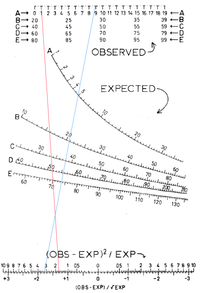
\includegraphics[width=0.25\linewidth]{dissertation//images//myFigures//design/200px-Chisquarenomo3.png}
    \caption{The nomogram of Pearson's Chi Square test \citep{boyd_nomogram_1965}}
    \label{fig:chi-square}
\end{figure}


As discussed in \Cref{background} and can be seen in \Cref{fig:chi-square} , nomograms can consist of axes in various shapes: lines, curves, arcs, etc. To create an accurate representation of the axis digitally, we need to find a general approach that can meet this requirement in an accurate way that is also intuitive and user-friendly. As there are many types of nomograms, a key goal was to represent a wide variety of nomograms in the application so that users could have complete freedom over the nomogram they wanted to interact with. On any nomogram a user wants to interact with, they should be able to select the shape of the axis, the range and scaling of the values on the axis, and the type of probability distribution they want to integrate for a missing value. 

There are several potential approaches to do so: 
\begin{enumerate}
    \item Using image contour detection to find the largest contour, 
    \item Highlighting an axis using a digital pen,
    \item Using Bézier curves
\end{enumerate}

Automatically finding the axis by sorting by the size of the contours on the nomogram would be the most convenient; however, this approach is prone to failure in many ways, including but not limited to false detections of nomogram instructions, legends on the graph, titles and labels, numbers and tick marks on the axes, etc. Using a lasso selection tool can limit false detections, but this can also lead to false detections, as described in \Cref{spec-problems}. 
Highlighting an axis with a digital pen would be the quickest way to minimise false detections. However, this approach can lead to significant inaccuracies and compounding errors.    

The third approach would be using Bézier curves, which are  
parametric curves commonly used in computer graphics. This was chosen as the basis for selecting axes on the nomogram, as explained in \Cref{nomo-logic}. Bézier curves provide a viable approach to accurately represent many different types of axes as they are defined through a series of control points. Let's define a  \textit{control point} as a point \(P\) that defines a Bézier curve, as shown in \Cref{fig:bezier-diagram}, and an \textit{axis (data) point} as the value of a variable on the axis of the nomogram on the Bézier curve. 

\begin{figure}[H]
    \centering
    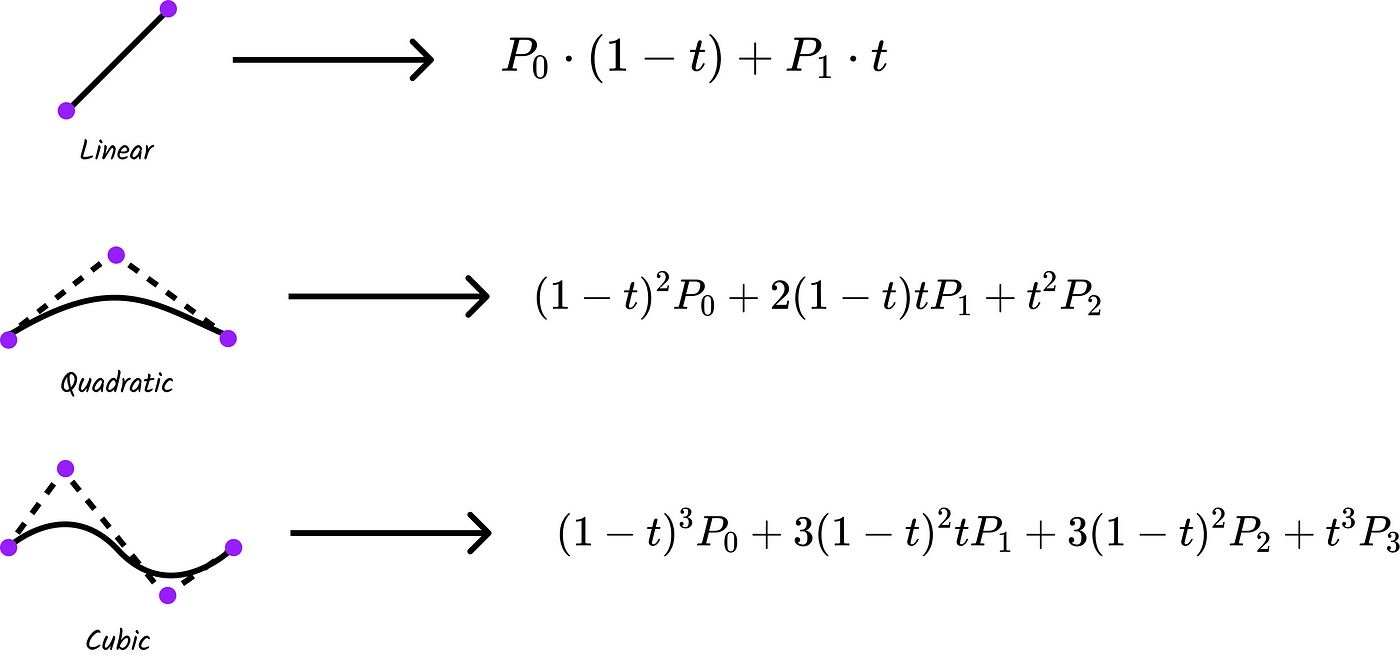
\includegraphics[width=0.875\linewidth]{dissertation//images//myFigures//design/bezier_control_points.png}
    \caption{A Bézier curve with \textit{n} \(\geq2\) control points produces a line or a polynomial of degree \textit{n-1} and the equation of the curve. Moving control points adjust the curvature according to the relative locations of the control points, as defined in \Cref{bezier-equation}. 
    \citep{melo_understanding_2021}}
    \label{fig:bezier-diagram}
\end{figure} 

The general parametric equation for a Bézier curve is as follows: 

\begin{equation}
\mathbf{B}(t) = \sum_{i=0}^{n} \binom{n}{i} (1-t)^{n-i} t^i \mathbf{P}_i
\label{bezier-equation}
\end{equation}
\begin{flushleft}
where $i$ represents the index of the control point, ranging from $0$ to $n$, and $t$ is the parameter that varies from $0$ to $1$, indicating the position along the curve.
\end{flushleft}

As users select more control points, the degree of the Bézier curve, denoted by $n$, increases, allowing it to accommodate more complex shapes and provide a more accurate representation of the axis. This improved accuracy stems from the inherent nature of polynomial fitting used in Bézier curves. As $n$ increases, the Bézier curve can better approximate intricate curves due to the increased accuracy afforded by higher-degree polynomials corresponding to higher-order Taylor expansions. Users can effectively reduce inaccuracies in the axis representation by selecting more control points and increasing the degree of the Bézier curve. This flexibility will enable finer adjustments and smoother transitions between control points, resulting in a curve closely matching the desired shape.  Each axis on the nomogram was designed to be generated by passing in an array of control points. If the user moves the control points, mouse event handlers should call relevant methods to update the axis. 

\subsection{Fitting of Data Points}

To facilitate the visualization of isopleths and their intersections, the program requires knowledge of the values on the axes at various points. Since the scaling of these values can vary greatly, ranging from linear to logarithmic, trigonometric, or even custom scales, a flexible method for calculating these values was designed.

One approach to achieve this flexibility is to ask the user to input four data points along each axis. These data points serve as reference values that define the scaling of the axis. By obtaining these reference points, the program can then interpolate or extrapolate the values at other points along the axis as needed.

For instance, if the user inputs four data points for the axis as $(x_1, y_1)$, $(x_2, y_2)$, $(x_3, y_3)$, and $(x_4, y_4)$, the program will use various mathematical techniques such as linear interpolation, logarithmic interpolation, or polynomial interpolation, to estimate the values at other points on the axis. This enables the program to accurately determine the coordinates of intersections and display the corresponding probabilities.


\subsection{Visualisations of Probability Distributions}

The method for visualizing probability distributions on different shapes of axes needs to be consistent to create consistent visualizations across various scenarios. Whether dealing with continuous or discrete distributions, maintaining coherence in visualization is essential for effectively communicating statistical information to a wide audience of users. 

For continuous distributions, such as the normal distribution or beta distribution, the parametrization of the curve allows for creating smooth, continuous visual representations. The resulting visualisations accurately portray the probability density function across the axis by generating ovals at each point along the axis, calculated through the continuous slicing of the $t$ value.

Similarly, the visualisation method remains consistent for discrete distributions like the binomial or Poisson distribution. Although discrete distributions involve specific individual points rather than a continuous curve, generating ovals at each point along the axis ensures uniformity in design. This consistency allows users to interpret and compare probability distributions across different scenarios and axis shapes seamlessly. 


\subsection{Data structures and Importing / Exporting Nomograms }

The application's main data structure was chosen as dictionaries that store the location of the nomogram, positions of the control points, the values of the axis, and the probability distributions for the axis, if any. Using dictionaries allows for quick access and a clear, logical structure. This way, users can share their configurations with others. The design of the data structures for the interactive application and the application save files were practically equivalent to making the implementation seamless. 

\section{User Interface}

The user interface was designed assuming most users did not know what a nomogram or Bézier curve was. Thus, they could learn the basics of nomograms and computer-aided geometric design to build and interact with probabilistic nomograms. 
\subsection{External consistency}

The user interface was designed so that the average user could load the image of a nomogram, select the shape of every axis, the range of the values on all axes and a probability distribution in less than ten minutes. The UIs of popular graph visualisation applications, such as Desmos and GeoGebra, were considered to explore interactive graphic calculators. Bezierve and Vernier Graphical Analysis were used to design the implementation of linear regression models on images combined with interactive visualisations. 
\begin{itemize}
    \item A toolbar with buttons to pick, load, and save projects, select control points, and enter probability distributions. 
    \item A side panel that shows the name of the axis, control points, and the probability distribution that can be scrolled.
    \item A canvas to view all graphical instruments and for interactions.
    \item An information panel on the bottom row of the application window to see the current mouse coordinates. 
\end{itemize}
 Selecting an ideal combination of icons for the toolbar proved challenging due to the unique requirements of this application, and a user study was necessary to evaluate the suitability of the selected icons for the application. 
\begin{figure}[H]
    \centering
    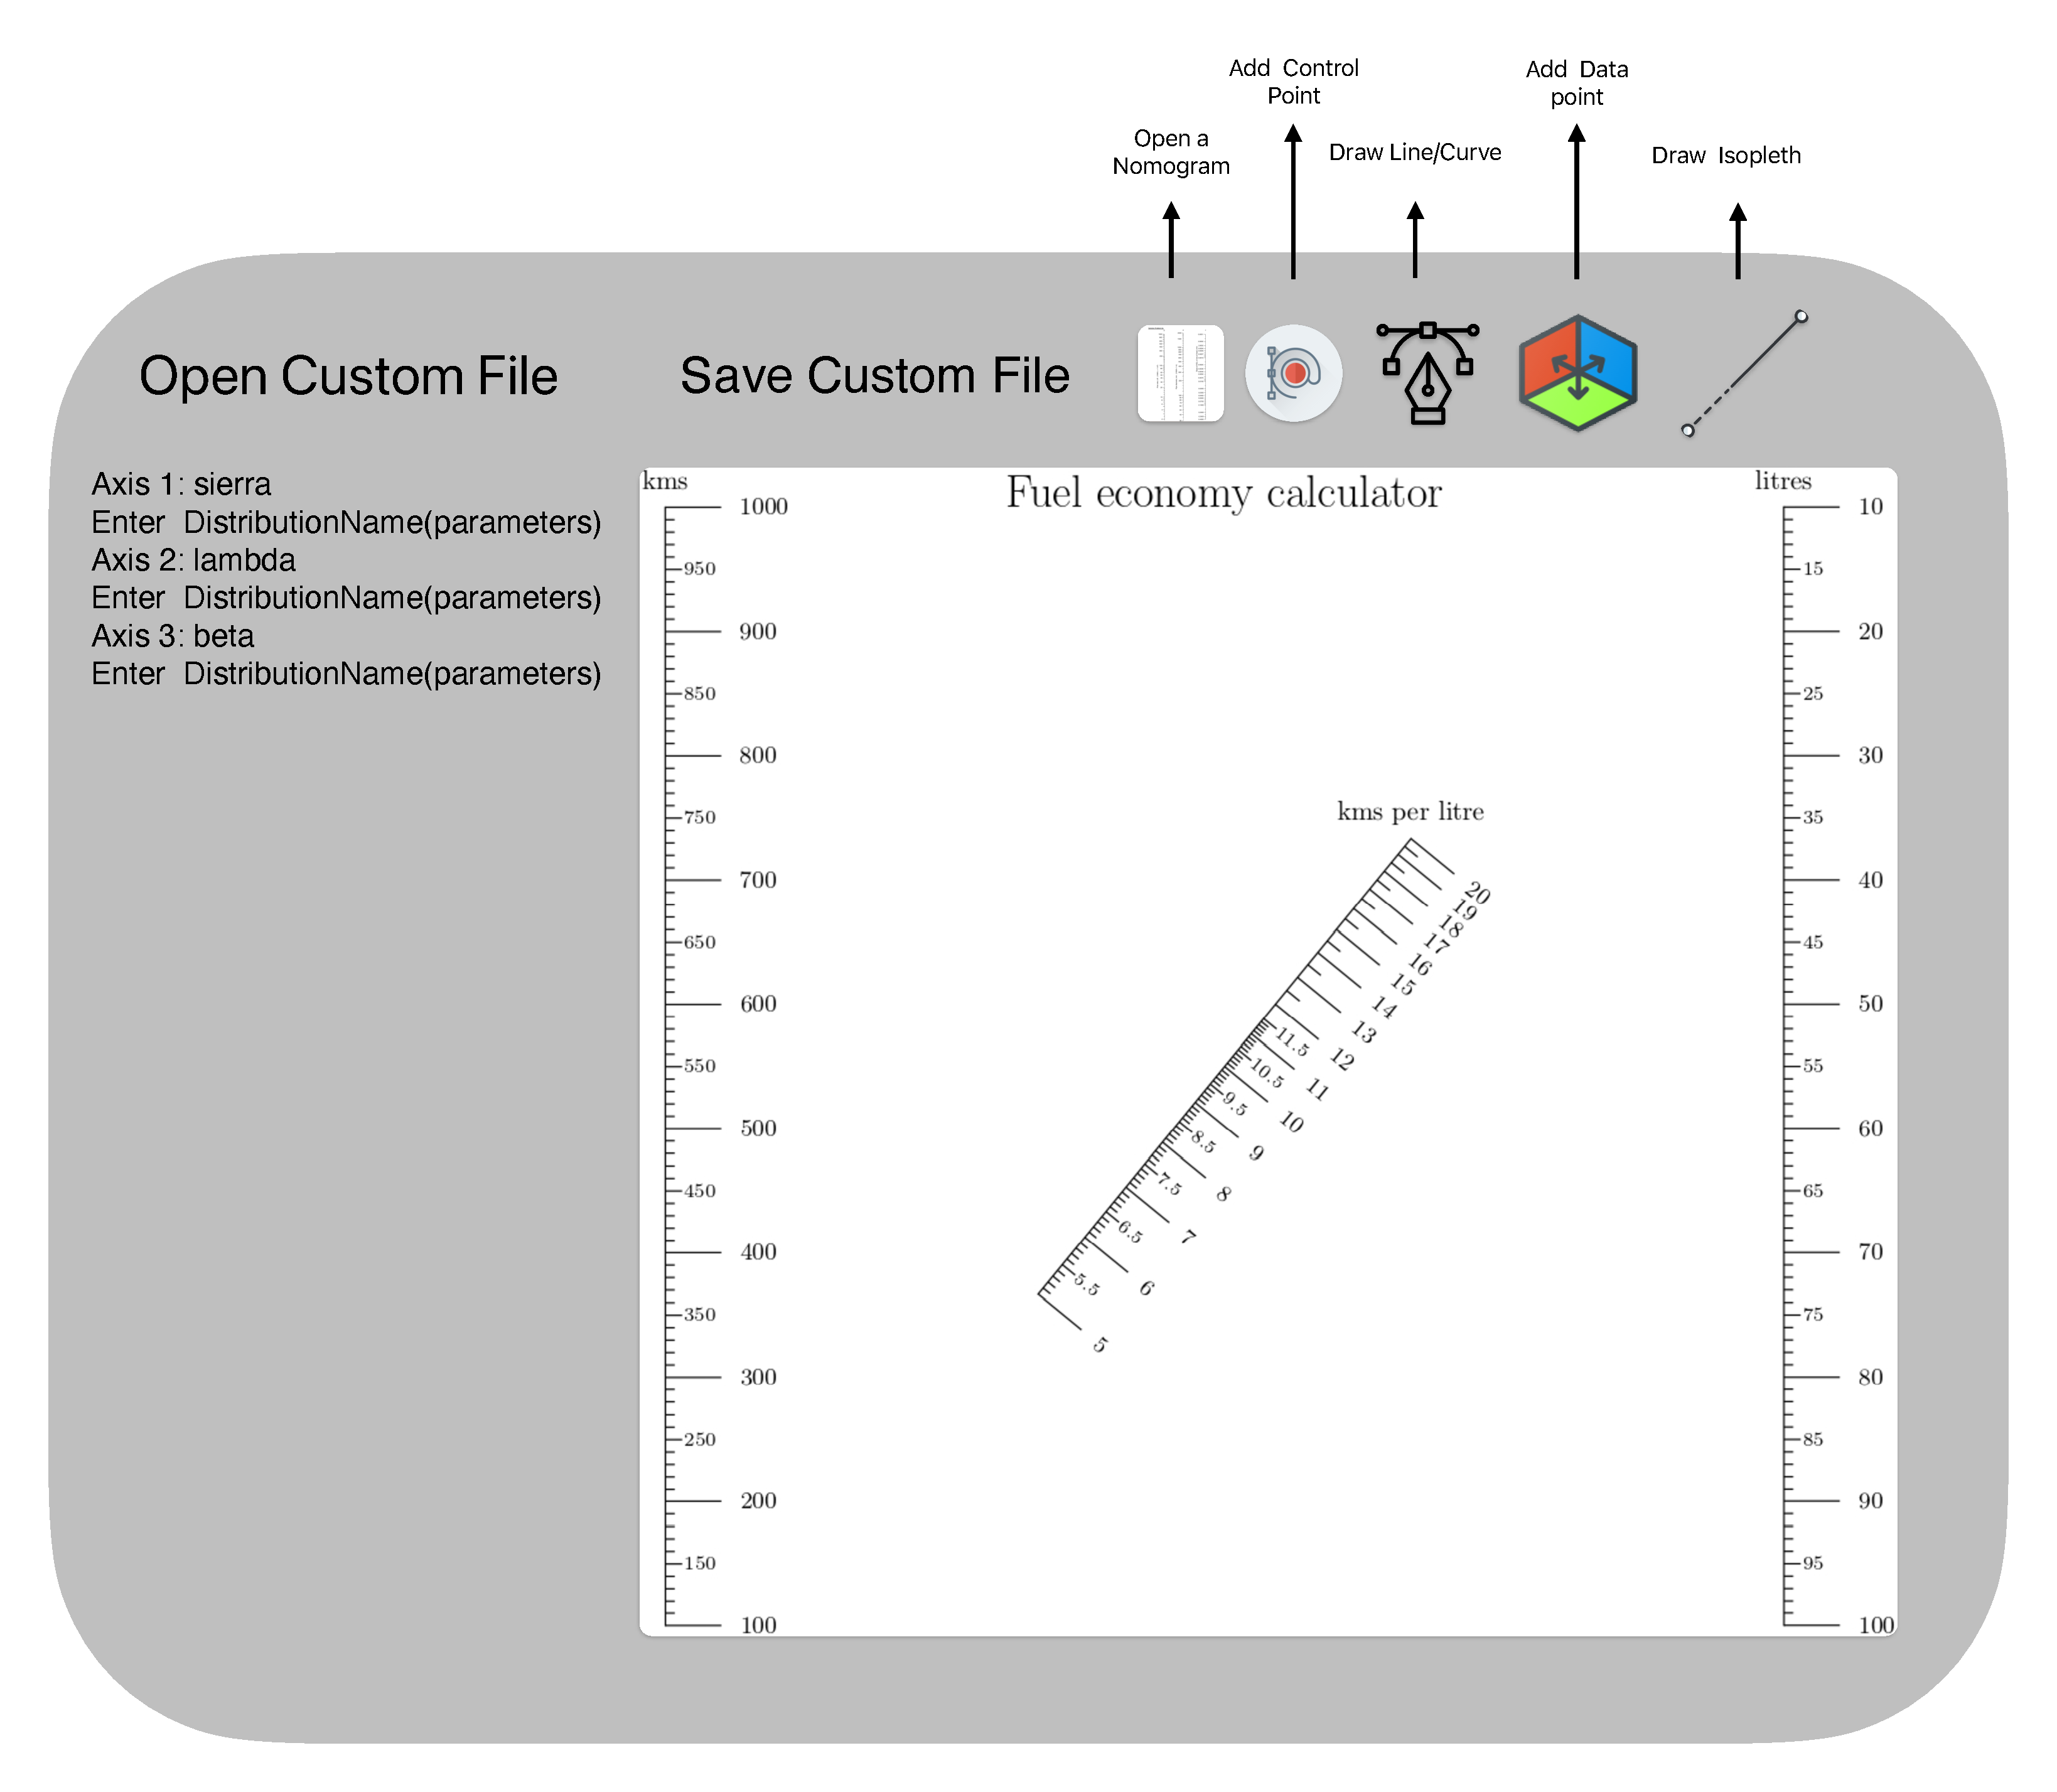
\includegraphics[width=1.3\linewidth]{dissertation/images/myFigures/design/wireframe.pdf}
    \caption{Initial program wire-frame shows the application's design before visualising probability distributions and user interaction with isopleths. The design has been revised during the implementation phase. }
    \label{fig:design-wireframe}
\end{figure}

%\section{Constraints in design} %

\section{Technologies}

\subsection{Python 3}
The programming language used for the application was chosen as Python 3 due to its popularity in the development of scientific calculations. Python 3 is multi-platform and is supported by all major operating systems and affordable single-board computers such as the Raspberry Pi. Python has a vast majority of libraries for drawing and interacting with Bézier curves, and calculations involving statistical distributions with SciPy and NumPy, which are well-developed with extensive built-in testing methods. Using Python allowed for the focus of development on the combination of features.

\subsection{Tkinter}

Tkinter is a built-in version of the Tk GUI in Python. It is included in all Windows, macOS, and Linux Python installations. Tkinter has a bu
ilt-in canvas that allows for event binding to mouse and keyboard movements, and it has extensive documentation to help solve complicated problems. The popularity of Tkinter in computing science education also means that most Python users can change the layout and the operation of the application without having to learn the additional know-how of other user interface frameworks such as PyQt. The combination of Python and Tkinter allows for producing portable application install files. 

\section{Application medium}

The project was designed to incorporate the benefits of paper-based nomograms, such as not requiring internet access while in use, portability, low cost, and ease of use. 
A desktop application was chosen as the suitable medium for development, as the chosen method of building a digital nomogram requires high accuracy with data input methods to compensate for the general disadvantages of nomograms. Even though there are more mobile phones than desktop computers in operation globally, mobile phones are difficult mediums to produce meaningful interactive visualisations on due to their small size, and a significant percentage of smartphones do not allow or make it difficult to use the Python packages chosen to develop this application.  

%==================================================================================================================================
\chapter{Implementation}\label{implementation}

The methods described in \Cref{design} have been implemented to create an accurate digital nomogram, using object-oriented GUI programming, where the main application class is the NomogramApp class. This class contains event handlers for mouse and keyboard interactions to satisfy the functional requirements by adjusting user mouse movements to contours on screen through the openCV library, as well as a dictionary which stores all axes in the nomogram: the control points, the axis points, the fitted equation for the axis, the probability distributions. The Isopleth class creates isopleths and shows details at intersection points. 

\begin{figure}[H]
    \centering
    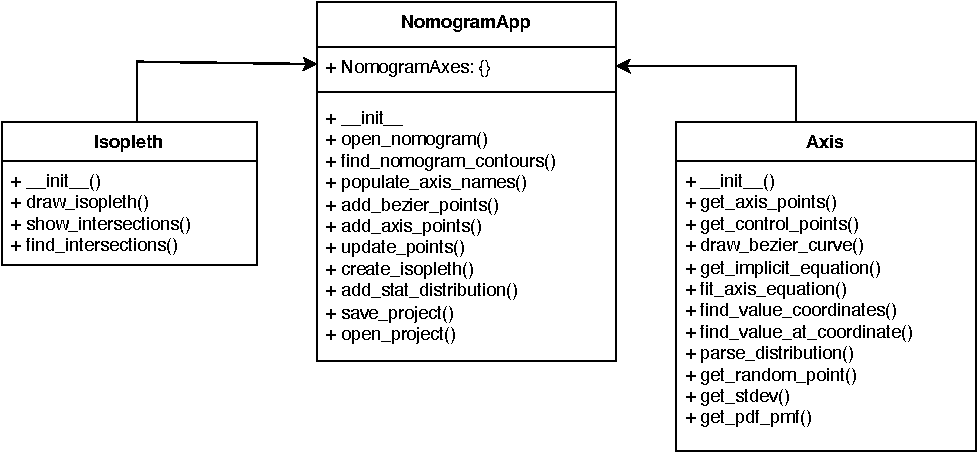
\includegraphics[width=\linewidth]{dissertation//images//myFigures//implementation/ClassDiagram.drawio.pdf}
    \caption{A simplified class diagram outlining the functions and methods created to implement the required features.}
    \label{fig:ClassDiagram}
\end{figure}

\section{User interface}

The user interface and the functionality to create digital representations of nomograms are operated using the built-in Python canvas. 

\section{Bézier curves} 

To find the most optimal implementation of Bézier curves in the application that justifies their selection and use ( which were the simplicity, accessibility, versatility, and precise control offered by Bézier curves ) and to represent all the different possible shapes of axes in nomograms, a comparison of available tools in Python led to the bezier package by \cite{hermes_bezier_2023} being picked due to its efficient implementation of the generation of the parametric equation of the Bézier curve using Fortran as a backend which is significantly faster than a native implementation in Python \citep{zwinkau_faster_nodate}, as well as the capability to generate an implicit function. The implicit function is an equation where the functional image of any coordinate on the Bézier curve \((x,y)\) equals zero. Combining the implicit equation with contour detection ensures that the movement of points on the canvas is bounded within a precise region, as described in \Cref{opencv-contour}. 



\section{Axis value}

A significant milestone in developing the application was creating a bidirectional conversion between a Cartesian coordinate on the canvas and the value on the axis. This is required so that probability distributions can be incorporated into the nomogram and intersections can be shown when an isopleth is moved. 

\subsection{From coordinates on the canvas to the axis}
To create a relationship between the geometric shape of the axis and its values, users must enter the values of four points to determine whether the axis is linear, logarithmic, or of another type. 

The discrete difference between the axis points entered by the user and the Euclidean distance of the coordinates on the canvas of these points is compared to classify an axis. If the difference is linear, then a linear fitting is applied. If the differences are reasonably logarithmic, a logarithmic scale is applied. Otherwise, a polynomial fitting of a second-order implicit equation is applied on the axis, and the equation coefficients are stored in the Axis object. 

Users can also add more data points to improve the precision of the fitting, and the predictions of five points are shown, calculated using the fitting function, as shown in  \Cref{fig:axis-equation-fitting}. 

\lstinputlisting[language=Python, caption=The implementation of the axis equation fitting in the application.]{dissertation//images//myFigures//implementation//codelistings/fittingfunction.txt
} \label{fig:axis-equation-fitting}


\subsection{From a point on the axis to the coordinate on the canvas}

Conversely, to display the value on an axis when a user drags an axis point or an isopleth, the fsolve method from the Scipy library was employed to find the root of the equation. This method utilizes a numerical approach to solve a pair of (non)linear equations, where one is the implicit equation of the Bézier curve, and the other is the difference between the axis value whose coordinates are to be found and the equation of the axis. The fsolve method returns a Cartesian coordinate when 

The fsolve function then iteratively refines an initial guess until a solution is found, making its steps using mathematical optimisation methods. \citep{virtanen_scipy_2020}

If the solution is successful, the method returns the determined coordinates (x, y) corresponding to the specified axis value. The solution is limited to the positive bounds of the width and height of the Tkinter canvas. 
\section{OpenCV Contour Detection} \label{opencv-contour}
\begin{figure}[H]
    \centering
    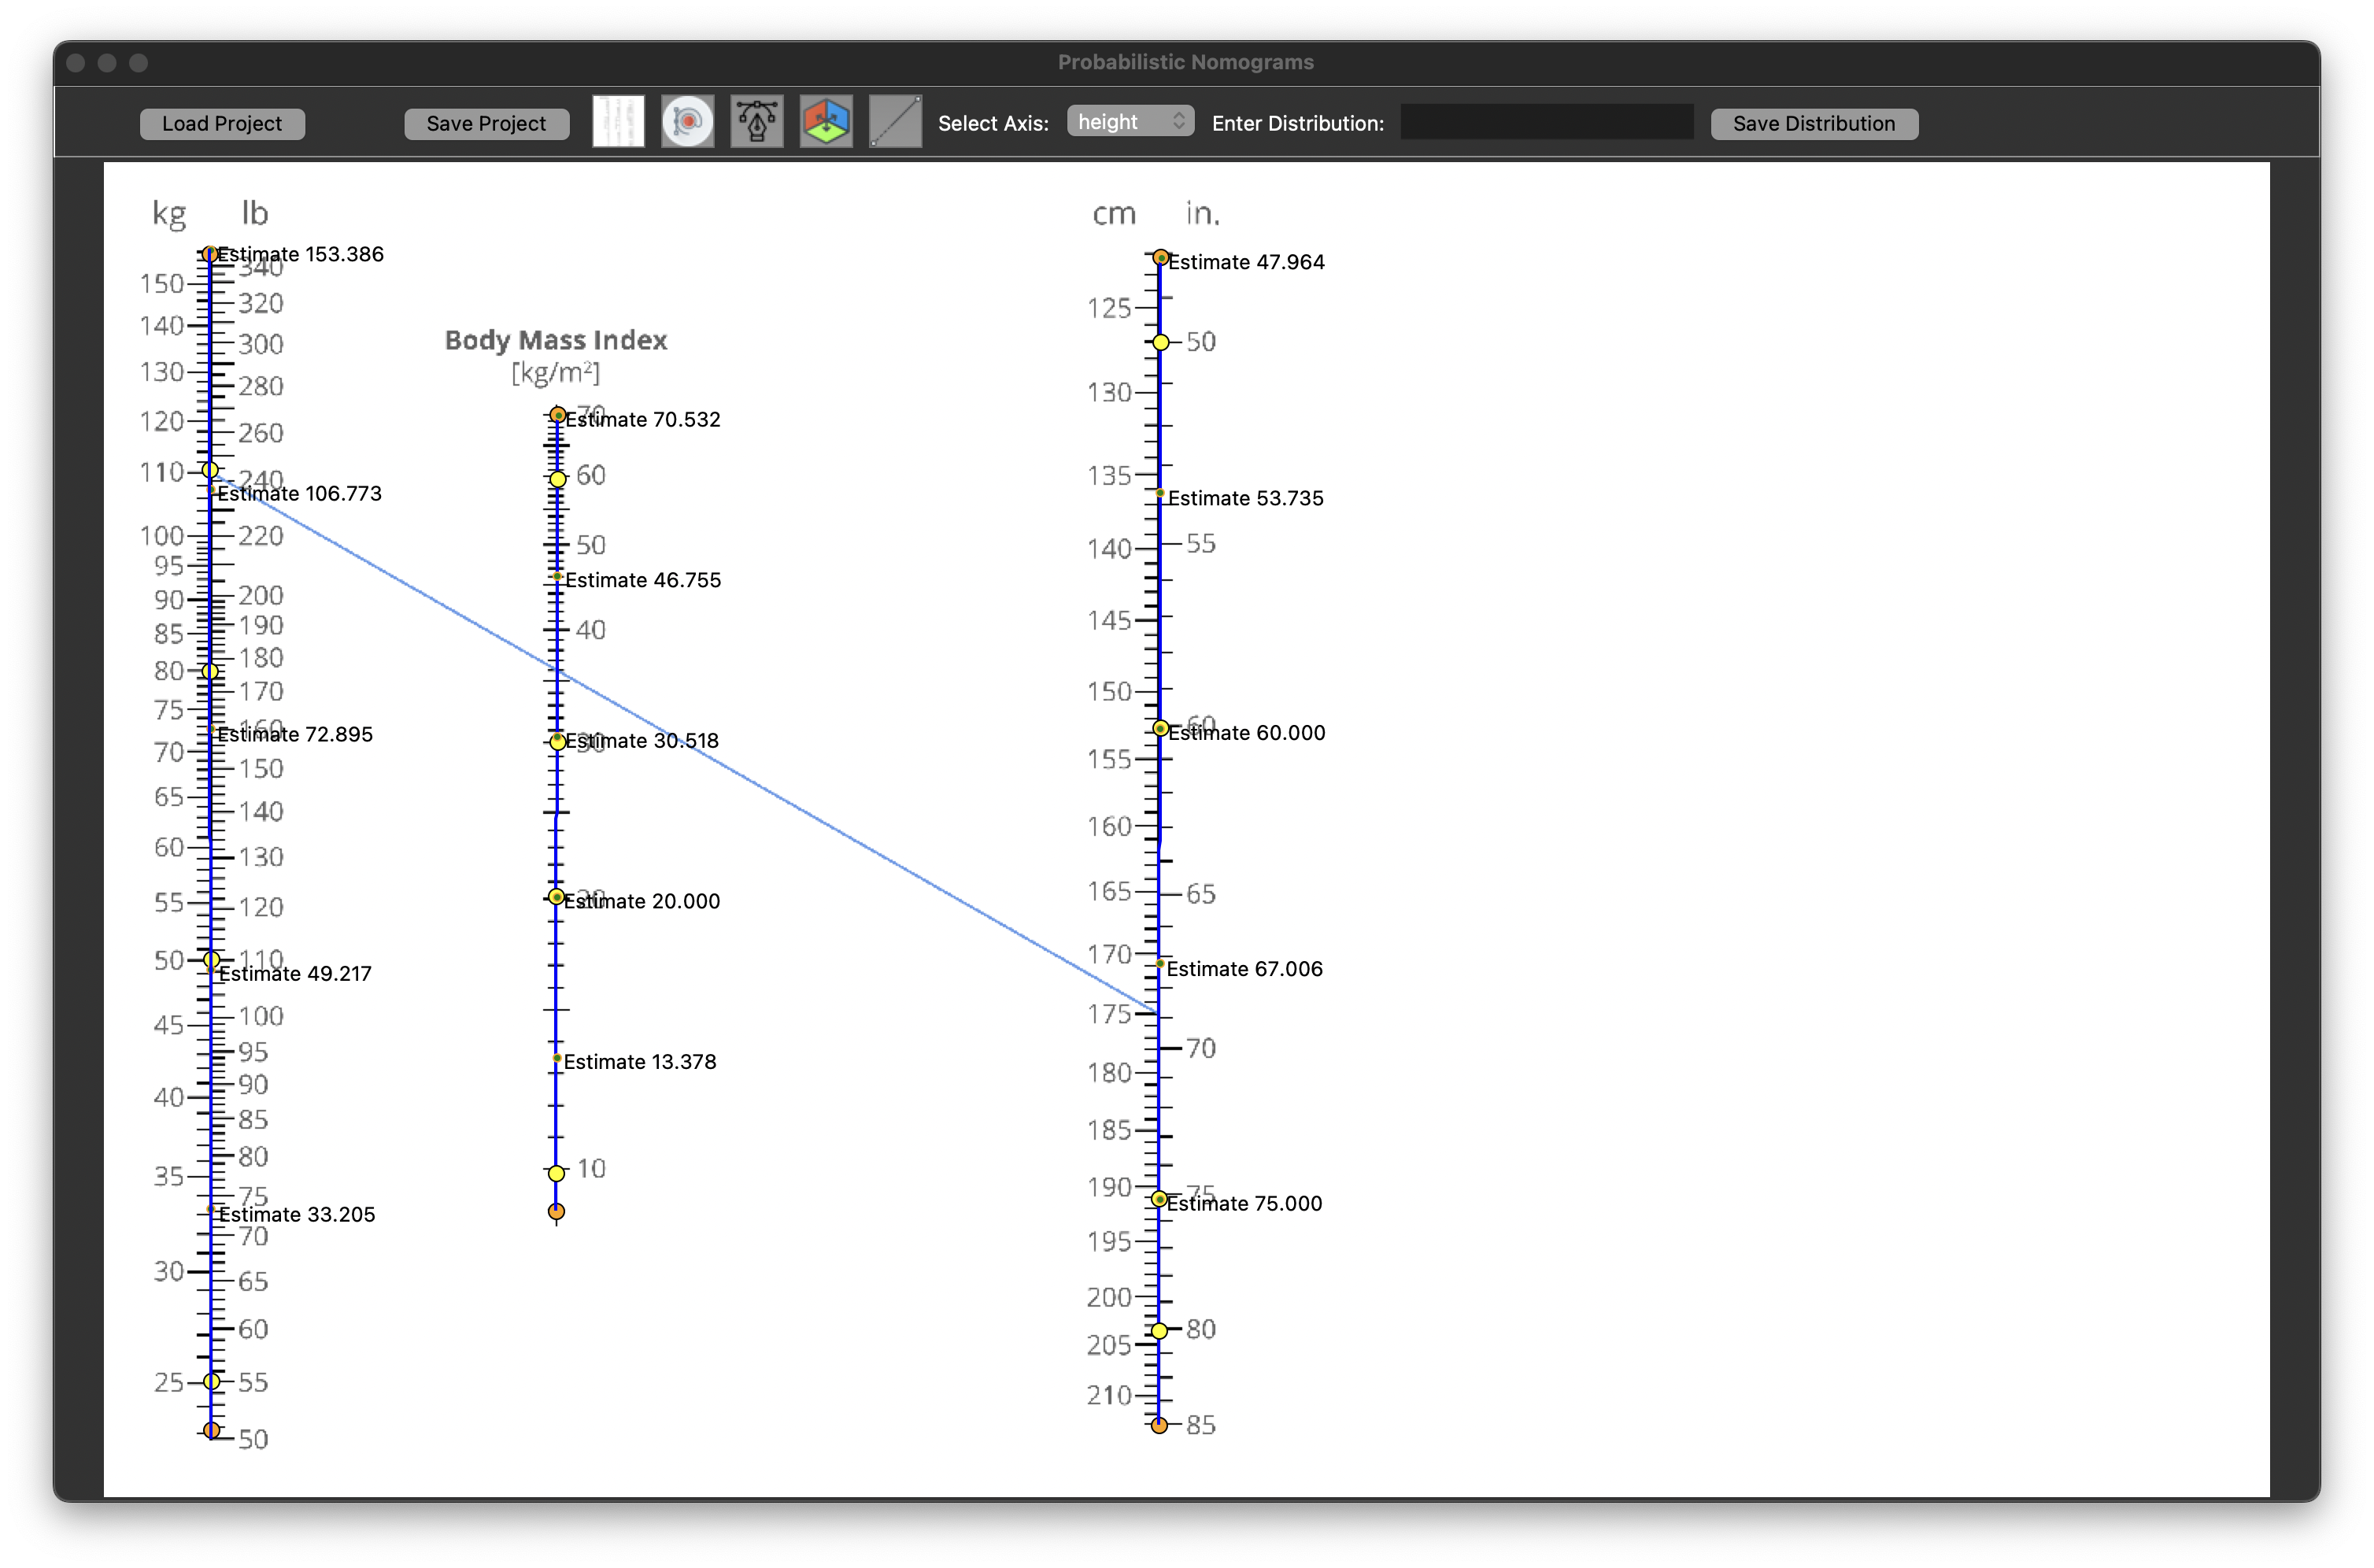
\includegraphics[width=\linewidth]{dissertation//images//myFigures//implementation/ss.png}
    \caption{The mouse event handler limits the movement of the control points of the Bézier curve to all contours on the image and the movement of the axis points to enter the values on the axis to the shape of the Bézier curve, drawn in blue. }
    \label{fig:complete-axis-screenshot}
\end{figure}
To minimize user error when selecting control points and axis points on a nomogram image, the OpenCV package was utilized to analyze the image and identify all the contours present. Contours represent the outlines of objects or shapes within an image and can be used to extract specific features or regions of interest.

Once the contours were obtained, the closest point function was implemented to automatically adjust the user's selection to the nearest contour point when they selected or moved a point on the nomogram. This approach aimed to improve user accuracy by aligning their input with the detected contours, thereby reducing the likelihood of selecting incorrect or unintended points.

A closest point function calculates the Euclidean distance between the mouse cursor position and the nearest contour point. If the distance to the nearest contour is below a threshold of 50 pixels, the optimal maximum distance from testing a range of thresholds, the user's selection is adjusted to coincide. This automatic adjustment significantly helps users align their selections with the detected contours, improving the precision of their input and reducing input error. 

However, suppose the distance between the cursor and the nearest contour point exceeds the predefined threshold, implying that the cursor is significantly distant from any contour point. In that case, the user's selection remains unchanged. This ensures that users can control their selections and freely adjust points when necessary, particularly for a nonlinear Bézier curve control point. The movement of the control points for an isopleth and the axis points are strictly limited to the Bézier curve of the axis, reducing the impact of compounding user input inaccuracies.


\section{Probability distribution integration}
\subsection{Importing probability distributions}
Probability distribution input text is parsed through regular expressions, as shown in \Cref{fig:regex-prob-dist}. The regular expression can easily detect the probability distributions and store the user-provided parameters as required by the Stats module from the SciPy library, which is dependent on the probability distributions, such as the mean of the distribution, the lower and upper bounds of the distribution, the degrees of freedom, the probability of success on trial, the number of trials, etc. Users can see these parameters from a tooltip when their mouse cursor hovers over the text input field. The list of probability distributions supported by the application can be seen in \Cref{fig:prob-tooltip}. 



\lstinputlisting[language=Python, caption=The implementation of the regular expression for parsing a probability distribution and its parameters., label=fig:regex-prob-dist]{dissertation//images//myFigures//implementation//codelistings/regex.txt
} 

\begin{itemize}
  \item \texttt{r}: Denotes a raw string. 
  \item \texttt{(\textbackslash w+)}: Captures the distribution name.
  \item \texttt{\textbackslash(}: Matches an opening parenthesis character \texttt{(} literally.
  \item \texttt{(.*?)}: Captures anything inside the parentheses non-greedily, representing the parameters.
  \item \texttt{\textbackslash)}: Matches a closing parenthesis character \texttt{)} literally.
\end{itemize}

The regular expression pattern captures the distribution name and its parameters enclosed in parentheses. This allows for flexibility in the input format, accommodating different distributions and their parameter styles. The captured groups can be further processed to extract the distribution name and parameters for statistical visualisations.

For example, if a user were to enter "Normal(50,3)", it assigns a Normal distribution with a mean of 50 and a standard deviation of 3 to that variable. 

\subsection{Visualisation of probability distributions}

To ensure the consistency of the visualisations of probability distributions across different shapes of nomogram axes, probability mass and density functions are drawn as a series of circles on points on the axes rather than traditional graphs of probability distributions, with the radius of circles being based on the probability density/ mass at that point, as shown in  \Cref{fig:prob-visualisation}. 

\begin{figure} [H]
    \centering
    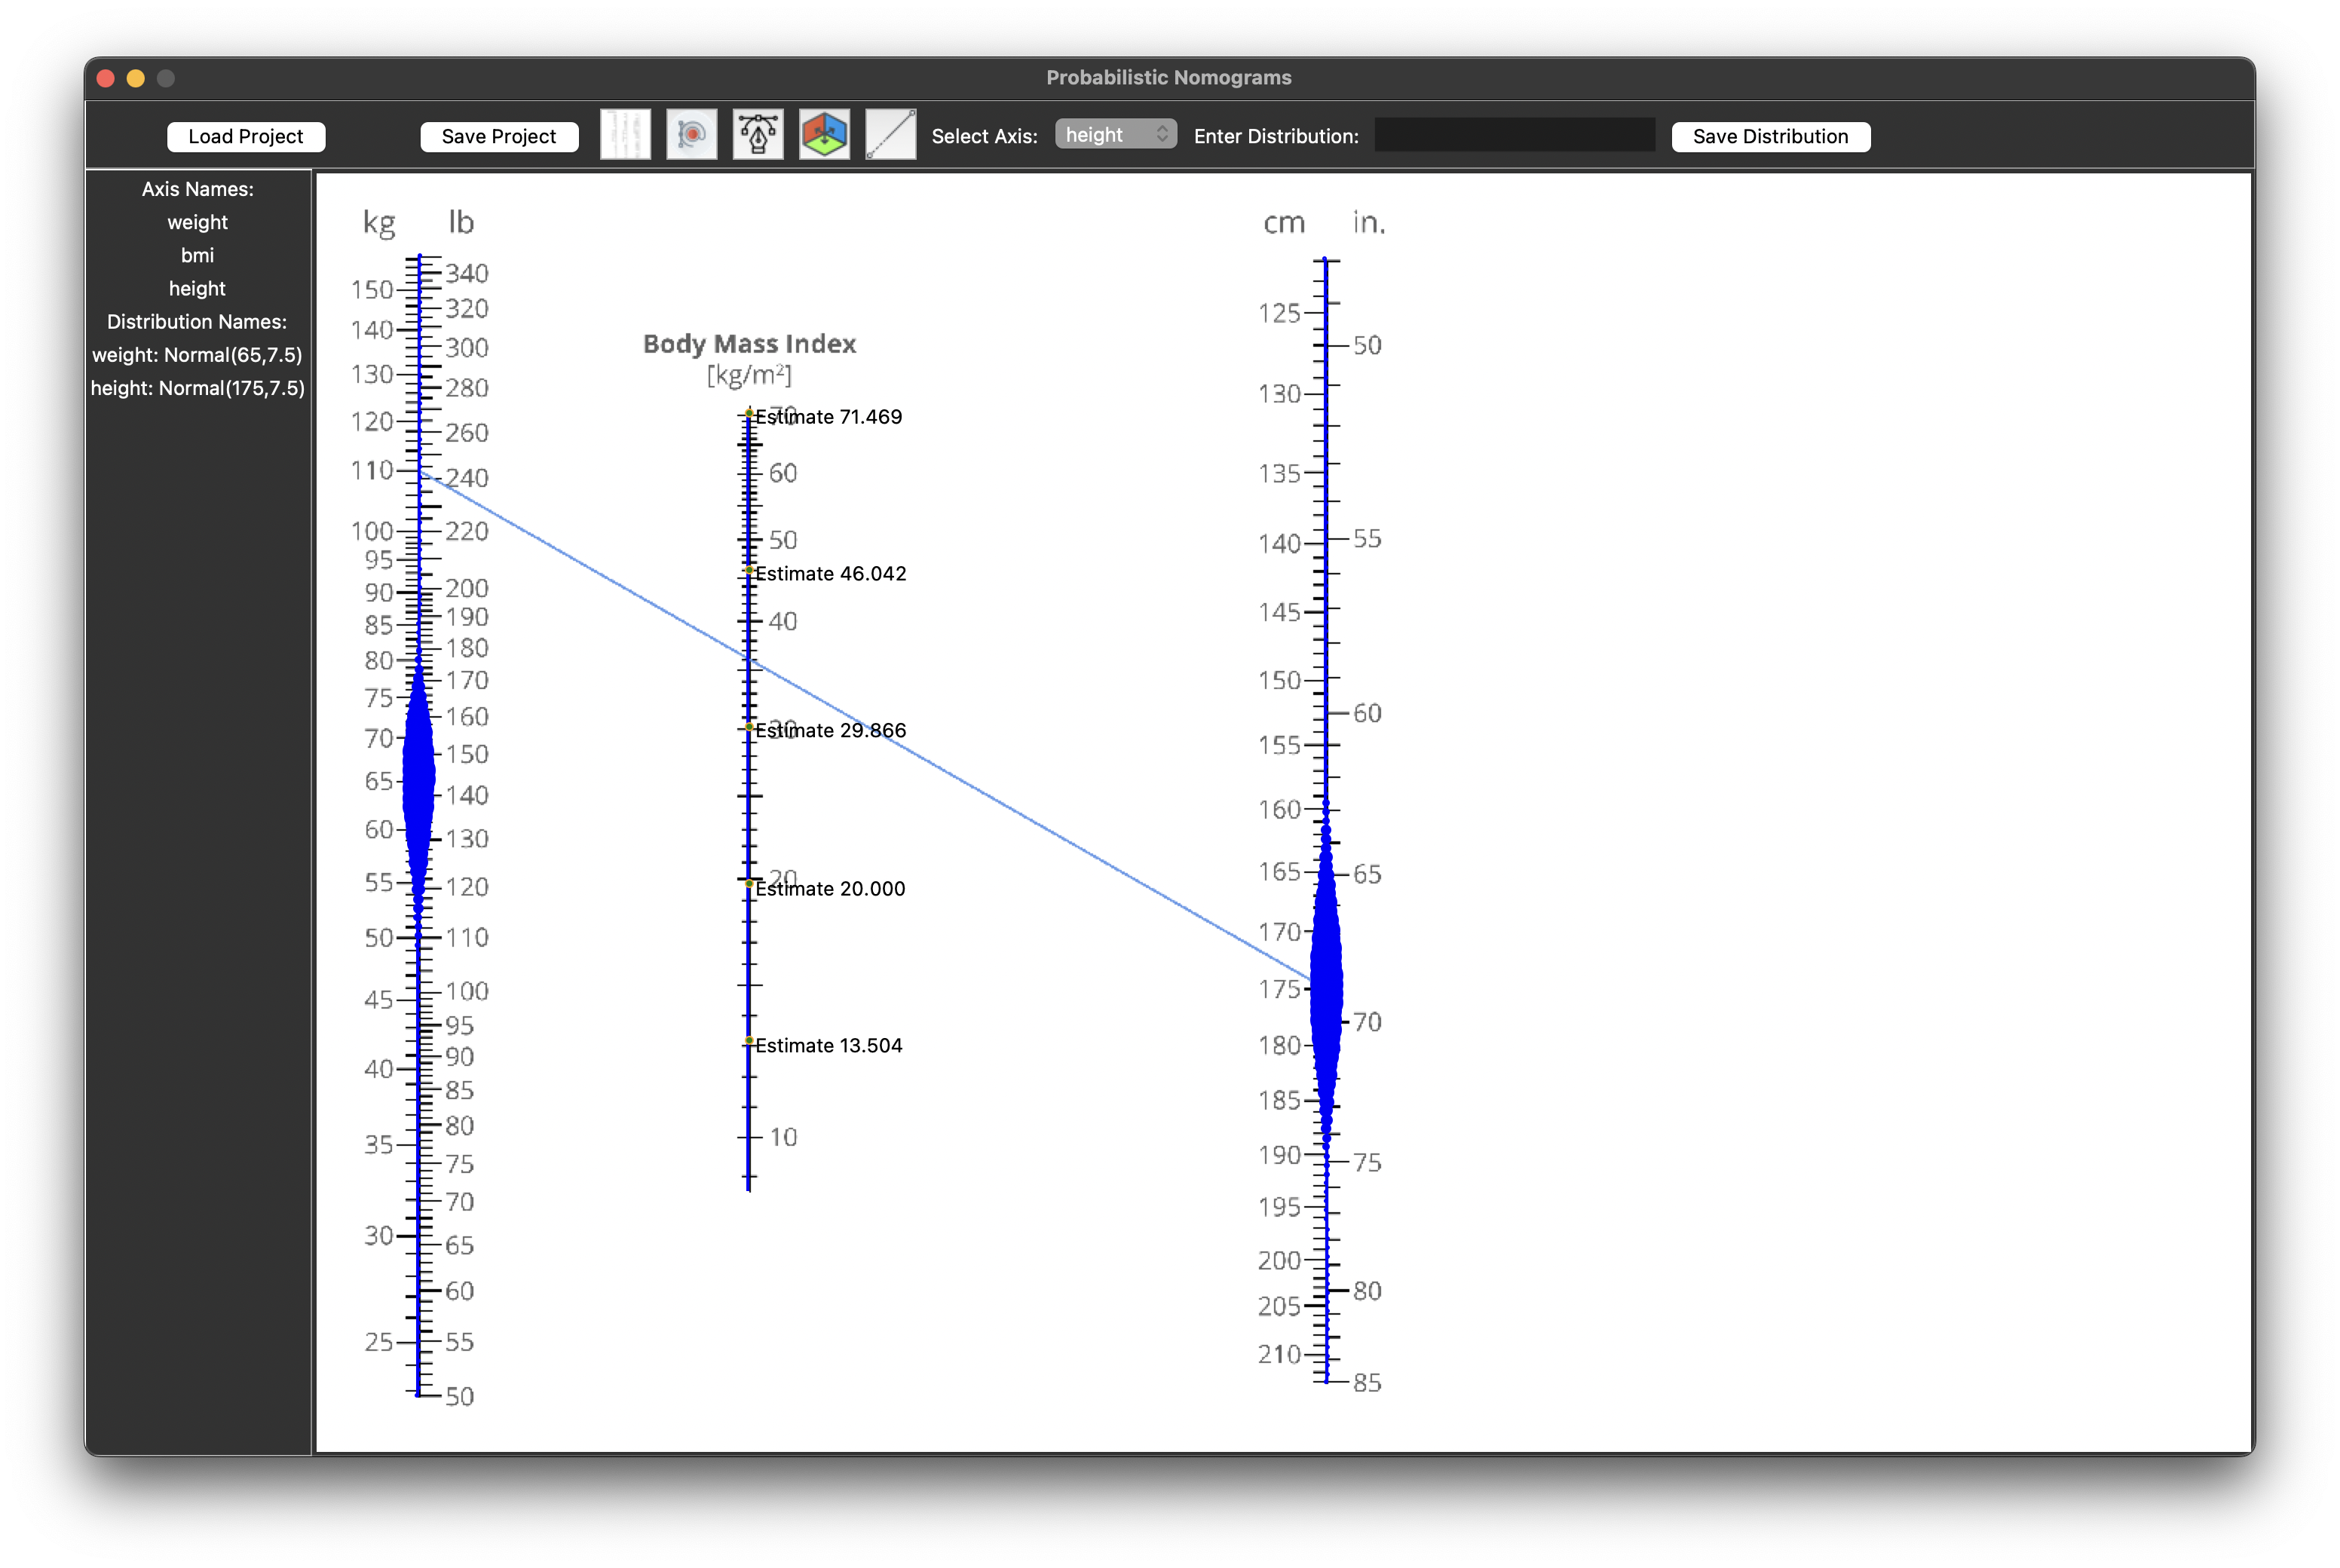
\includegraphics[width=0.75\linewidth]{dissertation//images//myFigures//implementation/probability1.png}
    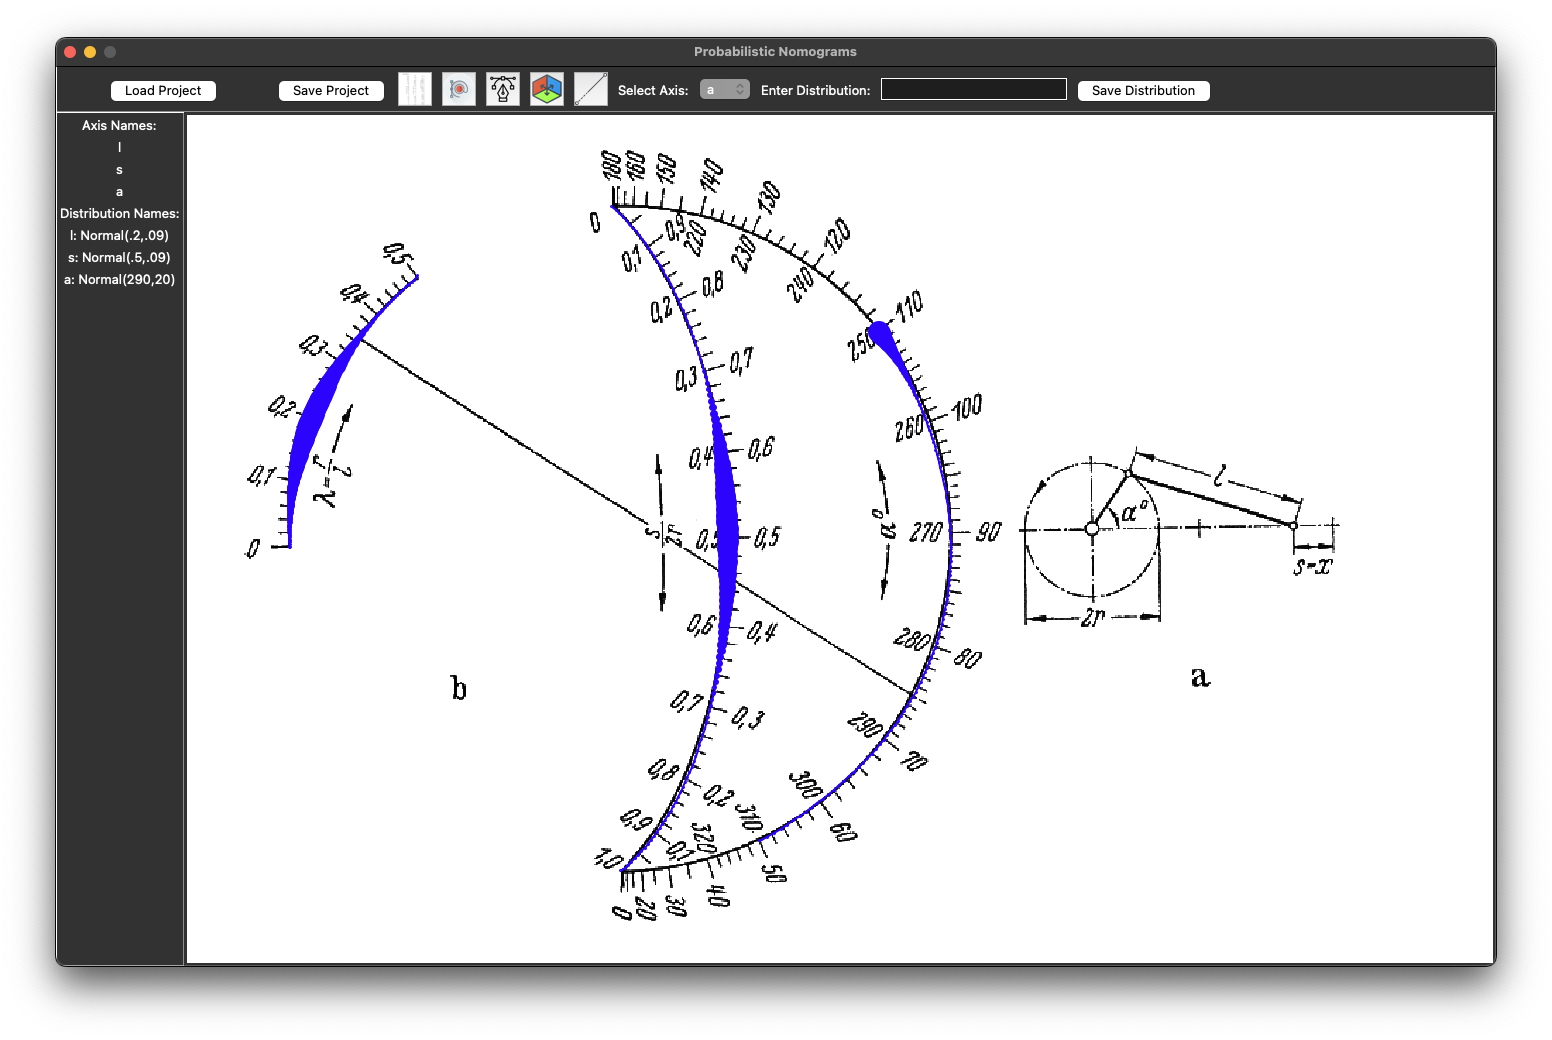
\includegraphics[width=0.75\linewidth]{dissertation//images//myFigures//implementation/probability2.png}    
    \caption{Two different nomograms consisting of axes with different shapes, visualising normal distributions.  }
    \label{fig:prob-visualisation}
\end{figure}

\section{Isopleth}

To create an isopleth, a furthest distance algorithm is run to find the axes of the nomogram that are the furthest from each other, and a random point is selected from the two axes. If a probability distribution represents the axis, the RVS method from Scipy.stats is the basis for the random point generator, which produces a random variate sample from the probability distribution, and the coordinate of this point is calculated. Otherwise, the Python built-in random number generator is used. These two random points are then treated as control points for a Bézier curve, producing a straight line that can be moved using the same event handlers as other points. The intersection is calculated using fsolve, Scipy's nonlinear equation solver, by looping through every axis and finding points whose implicit functions return zero. The probability value and the standard deviation are displayed next to the intersection point on the screen. 
\section{Importing and exporting files}

All generated nomograms can be exported and imported as JSON files that store all the control points, axis points, and probability distributions. This includes a reference to the directory of the image of the nomogram. 

\section{Deployment}

To deploy the application, the PyInstaller package was selected, which downloads all the required packages, including Numpy, Scipy, etc. so that users can run the application from a single application file. The drawback of this approach is that a different executable is required for each operating system, which reduces the portability of the application. The PyInstaller method runs on the GitHub continuous integration pipeline, developing a new executable every time new features are added. 

The second way to deploy the application is to share the source code as a compressed folder. However, this approach requires access to the Internet to download the requirements. 
\section{Maintainibility}

A crucial objective of the project was to enable future developers to maintain and expand upon it easily. Below are the steps to ensure the codebase attains a quality level that facilitates this goal. 
\subsection{Documentation}
\textbf{Issue tracking} Since the project's launch on GitHub, issue tracking was implemented. Code commits were associated with an issue where relevant, accompanied by a brief message outlining the commit's intended purpose or the goal it aimed to achieve. This approach was adopted to assist future developers in comprehending the code base, addressing bugs, and integrating new features. 
\newline
\textbf{Developer readme} The project also includes a developer-oriented README file. This document provides detailed instructions on setting up the project for development and two alternative deployment methods. The inclusion of this README aims to simplify the process for future developers to generate new executable versions of the program.
\newline


%==================================================================================================================================
\chapter{Evaluation} \label{evaluation}

The evaluation was done in two ways: first, by conducting a monitored user evaluation to investigate the users' perception and knowledge of nomograms, their ability to digitise and interact with an existing nomogram, and their general experience with using the application; second, by evaluating the application's ability to create an accurate representation of existing nomograms by calculating the accuracy of the fitting of data points. 

\section{Monitored user test} 

The monitored user test aimed to allow users to give feedback on the application's ease of use. The evaluation was monitored in anticipation of nomography's low spread across the wider population, allowing participants to ask questions if they were stuck during the testing. The users who participated were computing science students due to computing science students' frequent use of statistics and mathematics at university and in everyday life. 

\subsection{Task explanation}

\subsubsection{Task 1} consisted of building a digital representation of a body mass index(BMI) nomogram. This nomogram only has three axes: a person's body mass, height and body mass index. All axes have the shape of a line that only requires two control points to be generated, although more control points can be added. First, the participants had to open the provided BMI nomogram file. Then, the participants had to enter the names of the axes in the nomogram. Afterwards, they were instructed to add control points and create a Bézier curve for each axis to create an accurate overlay, adjusting the positions of the control points by dragging them as required. Then, they were instructed to add data points on each axis by selecting a coordinate and entering its value on the nomogram until the predictions produced by the axis equation fitting function were accurate and similar to \Cref{fig:complete-axis-screenshot}. 
\begin{figure}[H]
    \centering
    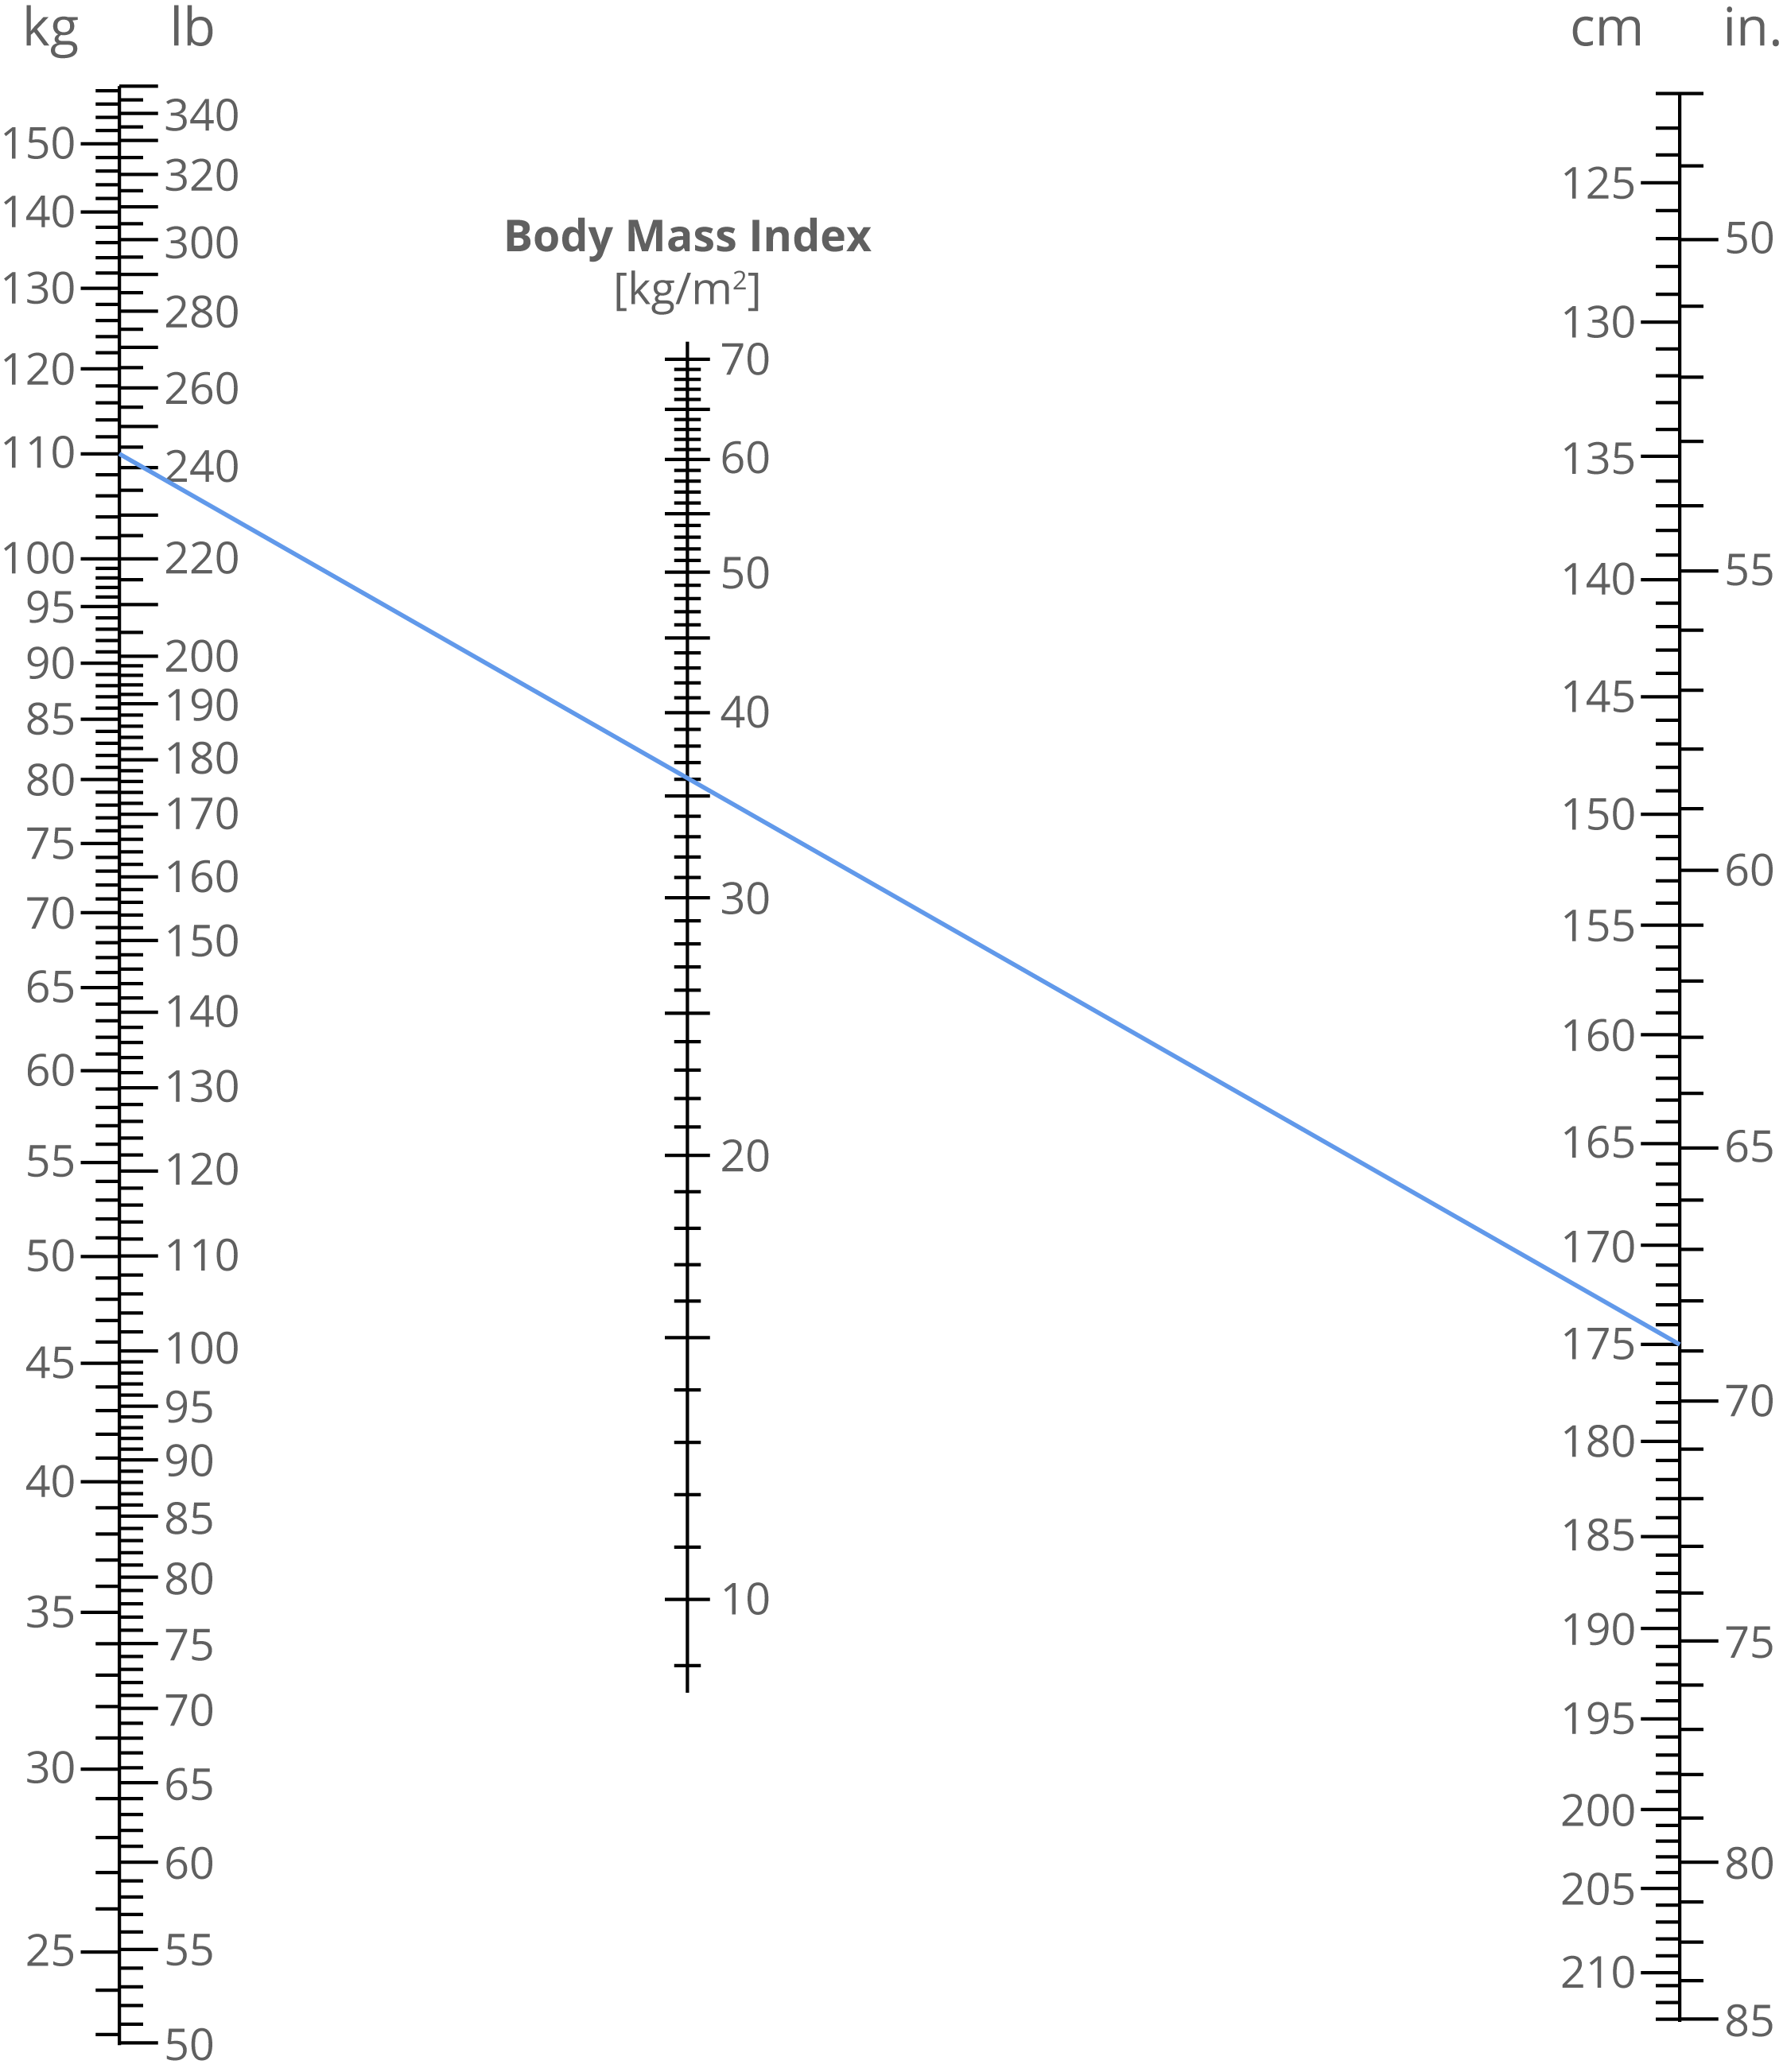
\includegraphics[width=0.8\linewidth]{dissertation//images//myFigures//appendix/bmi.png}
    \caption{The body mass index nomogram is used to calculate the body mass index of a person. All three axes have logarithmic scaling. \citep{merson-davies_body_2020}}
    \label{fig:bmi-nomogram}
\end{figure}
\subsubsection{Task 2} consisted of adding a probability distribution for two axes on the body mass index nomogram and interacting with the nomogram by moving an isopleth to read off-axis values from the interceptions and interpreting the probabilities. The users were given two normal distributions with a prepicked mean and standard deviations that they were to enter into the text field for the Add Distribution component. Then, they were instructed to add an isopleth and move its control points, where they could see the probability density, the standard deviation and the value of the interception point on the axis. 

\subsection{Monitoring}

The monitoring allowed users to get assistance while building a digital representation of nomograms, as the evaluation was designed for users who did not know about nomograms previously. 

\subsection{Evaluation questions}
For each task, users were asked how well they could perform the individual tasks, ranging from extremely well, somewhat well, neutral, somewhat not well, or extremely not well. They were also asked what improvements could be made to the application's workflow or if they had any technical problems while using it. For the control points or axis points entry, they were asked how many points they had to add to create an accurate digital representation of the nomogram. Users were also asked about their frequency of use of interactive graphical applications, how much they knew about nomograms, and where they see it plausible to use nomograms in their day-to-day activities. The full survey and answers are included in the \Cref{appendices} section. 

\subsection{Results}

\subsubsection{Qualitative results}
\begin{table}
\small
\centering
\begin{tabular}{|l|p{0.8\linewidth}|}
\hline
\textbf{ID} & \textbf{If you had any other difficulties while creating a digital representation of the nomogram, please explain them here.} \\ \hline
Participant 1 & Just remembering the instructions and commands, since it is the first time using the application \\ \hline
Participant 2 & Suggestion: allow the buttons to be toggled on or off \\ \hline
Participant 3 & The keyboard shortcuts weren't working well, but I realized that's because it was a Mac keyboard. There was a lot of button pressing repetition \\ \hline
Participant 4 & Remembering the shortcuts was difficult (though this would ease with time). I think the pictures at the top could be made slightly more intuitive. \\ \hline
Participant 5 & It would be nice to not have to click many times to add points of the same kind \\ \hline
Participant 6 & Sometimes assumed I could keep adding axis points without clicking the button again \\ \hline
Participant 7 & Instructions initially were unclear, but otherwise functionality was easy. \\ \hline
Participant 8 & Wasn't sure exactly what I was doing at first - I didn't know what a control point was and why I was putting them on the axis \\ \hline
Participant 9 & N/A \\ \hline
Participant 10 & Only issues stemmed from me not knowing nomograms \\ \hline
\end{tabular}
\caption{Summary of user feedback describing the challenges users faced when trying to create a probabilistic BMI nomogram shown in \Cref{fig:bmi-nomogram}.}
\label{fig:quali-eval-results-table}
\end{table}

\subsubsection{Suggested improvements to the program:}

\begin{enumerate}
    \item Incorporate an interactive tutorial at the program's launch to provide clear and concise guidance so that users can navigate the application that shows the user process interactively upon launching the application for the first time. These tutorials will walk users through essential functionalities, explaining each step with clear instructions and visual aids. By allowing users to interact with the tutorials, they can learn by doing, which enhances comprehension and retention of information.
    
    \item Implement a user-friendly interface with intuitive controls to alleviate cognitive burden: Redesign the interface to prioritize simplicity and ease of use. Utilize intuitive controls such as buttons, sliders, and drop-down menus that users can easily understand and navigate without extensive prior training. By reducing the cognitive load required to operate the application, users can focus more on their tasks and less on deciphering complex commands.
    
    \item Introduce toggling buttons for greater flexibility and customization in the user interface: Allow users to toggle various features or settings according to their preferences. Toggling buttons would allow users to save time by not having to press a button repeatedly. 

\end{enumerate}


\textbf{Ease of use }

Participants 1, 3, 4, and 5 felt they could create an accurate representation of the nomogram on the canvas to some extent.

Participants 2, 6, 7, 8, 9, and 10 expressed that they were extremely skilled at creating an accurate representation of the nomogram on the canvas.

Overall, while some participants found it somewhat challenging to create an accurate representation, a majority felt they were able to do so extremely well, which shows that some improvements are necessary to improve the user interaction and the fitting of the axis data points. 

\textbf{Usefulness as a learning tool}

The responses indicate a mixed but generally positive perception of nomograms as a tool for creating interactive visualizations of calculations. Participants who expressed interest in using nomograms for this purpose recognized the value of visual representations in enhancing understanding and facilitating analysis.

The applications varied widely for those who indicated they would use nomograms to create interactive visualizations. Some participants mentioned specific domains such as car fuel efficiency, probability and statistical analysis equations, equations in experiments, and engineering calculations. 

\subsubsection{Limitations}

The study participants were fourth-year computing science students who have much more technical skills than the average student. Thus, the participants involved in this study do not perfectly represent the target user demographic for the product being evaluated. 

Some participants had more extensive experience with mathematical concepts, including linear regression, due to their involvement in visual information interpretation-related computer science courses, as opposed to students who study cyber security or programming languages. 

While this variance in technical background was considered acceptable for the purposes of the study, as nomograms are not well known, it could have influenced participants' perceptions of the program's impact on their understanding of the subject matter. By including participants from social sciences backgrounds, the study could capture a more diverse range of user experiences and perspectives. These participants may approach the program with different levels of technical proficiency and familiarity with mathematical concepts.

Furthermore, participants from social sciences disciplines may offer unique insights into the program's usability in real-world scenarios relevant to their field of study. Their feedback could shed light on the program's practical applicability and effectiveness in supporting data analysis tasks commonly encountered in social sciences research. The choice of a BMI nomogram, which is not commonly used in computing science courses, was to strike a balance between the computing knowledge of the participants and the medical uses of BMI nomograms. 

\subsubsection{Quantitative results}

One participant experienced issues while using the program and, therefore, could not create an accurate representation of the axis on the nomograms. Therefore, their quantitative results have not been included.

\begin{table}[H]
\begin{tabular}{llll}
Participant \# / Axis & First axis (height)       & Second axis(BMI)          & Third axis(weight)        \\
Participant 1         & \cellcolor[HTML]{DDEBF7}4 & \cellcolor[HTML]{DDEBF7}4 & \cellcolor[HTML]{DDEBF7}4 \\
Participant 2         & 6                         & 6                         & 4                         \\
Participant 3         & \cellcolor[HTML]{DDEBF7}4 & \cellcolor[HTML]{DDEBF7}5 & \cellcolor[HTML]{DDEBF7}4 \\
Participant 4         & 4                         & 4                         & 4                         \\
Participant 5         & \cellcolor[HTML]{DDEBF7}4 & \cellcolor[HTML]{DDEBF7}4 & \cellcolor[HTML]{DDEBF7}4 \\
Participant 6         & 4                         & 4                         & 4                         \\
Participant 7         & \cellcolor[HTML]{DDEBF7}4 & \cellcolor[HTML]{DDEBF7}4 & \cellcolor[HTML]{DDEBF7}4 \\
Participant 8         & 4                         & 4                         & 4                         \\
Participant 9         & \cellcolor[HTML]{DDEBF7}4 & \cellcolor[HTML]{DDEBF7}4 & \cellcolor[HTML]{DDEBF7}4
\end{tabular}
\label{fig:quanti-eval-results-table}
\caption{The number of axis data points users had to add for each axis on the body mass nomogram shown in \Cref{fig:bmi-nomogram} to get an accurate fitting from the application. }
\end{table}

The quantitative results suggest that users found creating an accurate digital representation of the nomograms relatively straightforward once they understood the application's workflow. The fact that most participants could accurately represent the nomogram with the minimum required control points and axis data points indicates the effectiveness of the application's design and implementation and the effectiveness of the numerical methods used to combine the features. 

\section{Impact of Axis Data Points Selection}
\subsection{Task explanation}
Users exercise significant discretion in selecting the axis data points when fitting the values on an axis on a nomogram. The selection of the points significantly impacts the accuracy of the fitting, as picking points that are linearly distant on a straight-line axis with logarithmic scaling can cause the program to assume that the values on the axis have linear scaling. 

\subsection{Method}
Three nomograms with varying axis types were tested to evaluate the impact of the user's selection. This was done by manually creating a digital representation of the three nomograms to create an accurate representation, and after achieving an accurate fitting, by randomly picking four points with a corresponding axis value calculated from the true fitting equation, then attempting a fitting with those four random data points, and comparing the value of all true data points on the axis of the nomogram with all the values on the axis of the nomogram from the randomly generated fitting equation. The root mean square of the differences was calculated. Each test was done 10 times for every axis. 

\subsection{Results}
\begin{table}[h]
    \centering
    \begin{tabular}{lc}
        \toprule
        Axis Name & RMS Inaccuracy \\
        \midrule
        \texttt{Kilometres} & $2.252 \times 10^{-7}$ \\
        \texttt{Litres of petrol} & $3.675 \times 10^{-9}$ \\
        \texttt{Kilometres per litre} & $8.163 \times 10^{-9}$ \\
        \bottomrule
    \end{tabular}
    \caption{The RMS inaccuracy for the fuel efficiency nomogram in \Cref{fig:fuel-efficiency}}
\end{table}

\begin{table}[h]
    \centering
    \begin{tabular}{lc}
        \toprule
        Axis Name & RMS Inaccuracy \\
        \midrule
        \texttt{BMI} & $1.731 \times 10^{-8}$ \\
        \texttt{Height} & $3.920 \times 10^{-9}$ \\
        \texttt{Mass} & $1.550 \times 10^{-7}$ \\
        \bottomrule
    \end{tabular}
    \caption{The RMS inaccuracy for the BMI nomogram in \Cref{fig:bmi-nomogram}}
\end{table}

\begin{table}[h]
    \centering
    \begin{tabular}{lc}
        \toprule
        Axis Name & RMS Inaccuracy \\
        \midrule
        \texttt{$\lambda$} & $1.265 \times 10^{-5}$ \\
        \texttt{s} & $4.538 \times 10^{-4}$ \\
        \texttt{$\alpha$} & $1.910 \times 10^{-1}$ \\
        \bottomrule
    \end{tabular}
    \caption{The RMS inaccuracy for a slider-crank mechanism nomogram in \Cref{fig:slider-crank}}
\end{table}

It is clear from the testing that the accuracy of the fittings on axes which are not straight lines, as in \Cref{fig:slider-crank}, are significantly more dependant on the selection of the axis data points by a significant order of magnitude. There does not appear to be a significant difference between straight-line axes with linear and logarithmic scaling, which can be found in a higher number of nomograms.  

\subsubsection{Limitations}

While the results of this experiment show a significant difference in the RMS inaccuracies depending on the shape of an axis, this experiment is insufficient to determine the impact of the scaling on the axis themselves, as points have been selected randomly. A collection of data from a large set of users would be required to determine the impact of the choice of points on the fitting as well as users' understanding of the impacts of linear and logarithmic scaling on linear regression models, which was not evaluated and might be useful to do so for educational purposes. 

\section{Verification of program requirements}

\subsection{Functional requirements}

The first, third, fourth and fifth functional requirements were met through user testing. 
The second functional requirement was tested through automated tests but not user testing. User testing was intended to create interactive visualisations of nomograms with probabilistic relationships, and saving custom project files only restored the information entered by other users.

\subsection{Non functional requirements}
Both non-functional requirements have been met. 
\section{Automated user tests}
The Pynguin package in Python has been used to create automated testing for the application's individual classes, including the user interface and the input parameters and outputs for the various methods implemented. 

%==================================================================================================================================
\chapter{Conclusion}\label{conclusion}
In this project, we have developed an application to allow users to interact with nomograms where probability distributions can represent a variable instead of a fixed value, which creates uncertainty. This project was motivated by how nomograms provoke interest due to being unusual, helping people who would rather use pictures than calculators to develop an understanding of complex calculations as well as the challenges faced by students in solving probabilistic problems that are caused by procedural and technical errors due to a lack of experience. 

This application was developed through a series of data inputs, including creating Bézier curves to represent axes and entering data points for various points on the curve to create an accurate fitting.  Various optimisation methods were used to represent the many different types of nomograms that were present accurately. Probability distributions can be visualised and interpreted through consistent design elements. The effectiveness of the application was evaluated through user studies, where users were asked to create a digital representation of the body mass index nomogram, with the results suggesting that the approaches used were sufficient in creating accurate representations after understanding the concepts behind nomograms, Bézier curves, linear regression and the use of probability distributions. All of the functional and non-functional requirements of the application have been met. Quantitative evaluations have shown that the application is more suitable for nomograms where the axes are straight lines compared to curved axes due to the increased variability of the user selection of data points and their respective coordinates. 

The main drawback of the application was the user experience, which was challenging to design due to the unpopularity of nomograms and a lack of similar applications. 

\section{Future work}

Future work to improve this application includes but is not limited to:
\begin{enumerate}
    \item Improving the user experience by implementing easy-to-understand on-screen tutorials, binding controls to ensure a smooth operation,
    \item Ability to interpret nomograms from applications such as PyNomo,
    \item Support for additional probabilistic methods, such as importing custom datasets,
    \item Improved models for data fitting by testing with more nomograms, 
    \item User evaluations in primary and secondary school settings to gather more feedback. 
    
\end{enumerate}

%==================================================================================================================================
%
% 
%==================================================================================================================================
%  APPENDICES  

\begin{appendices}

\chapter{Appendices}\label{appendices}




\section{Ethics checklist}
    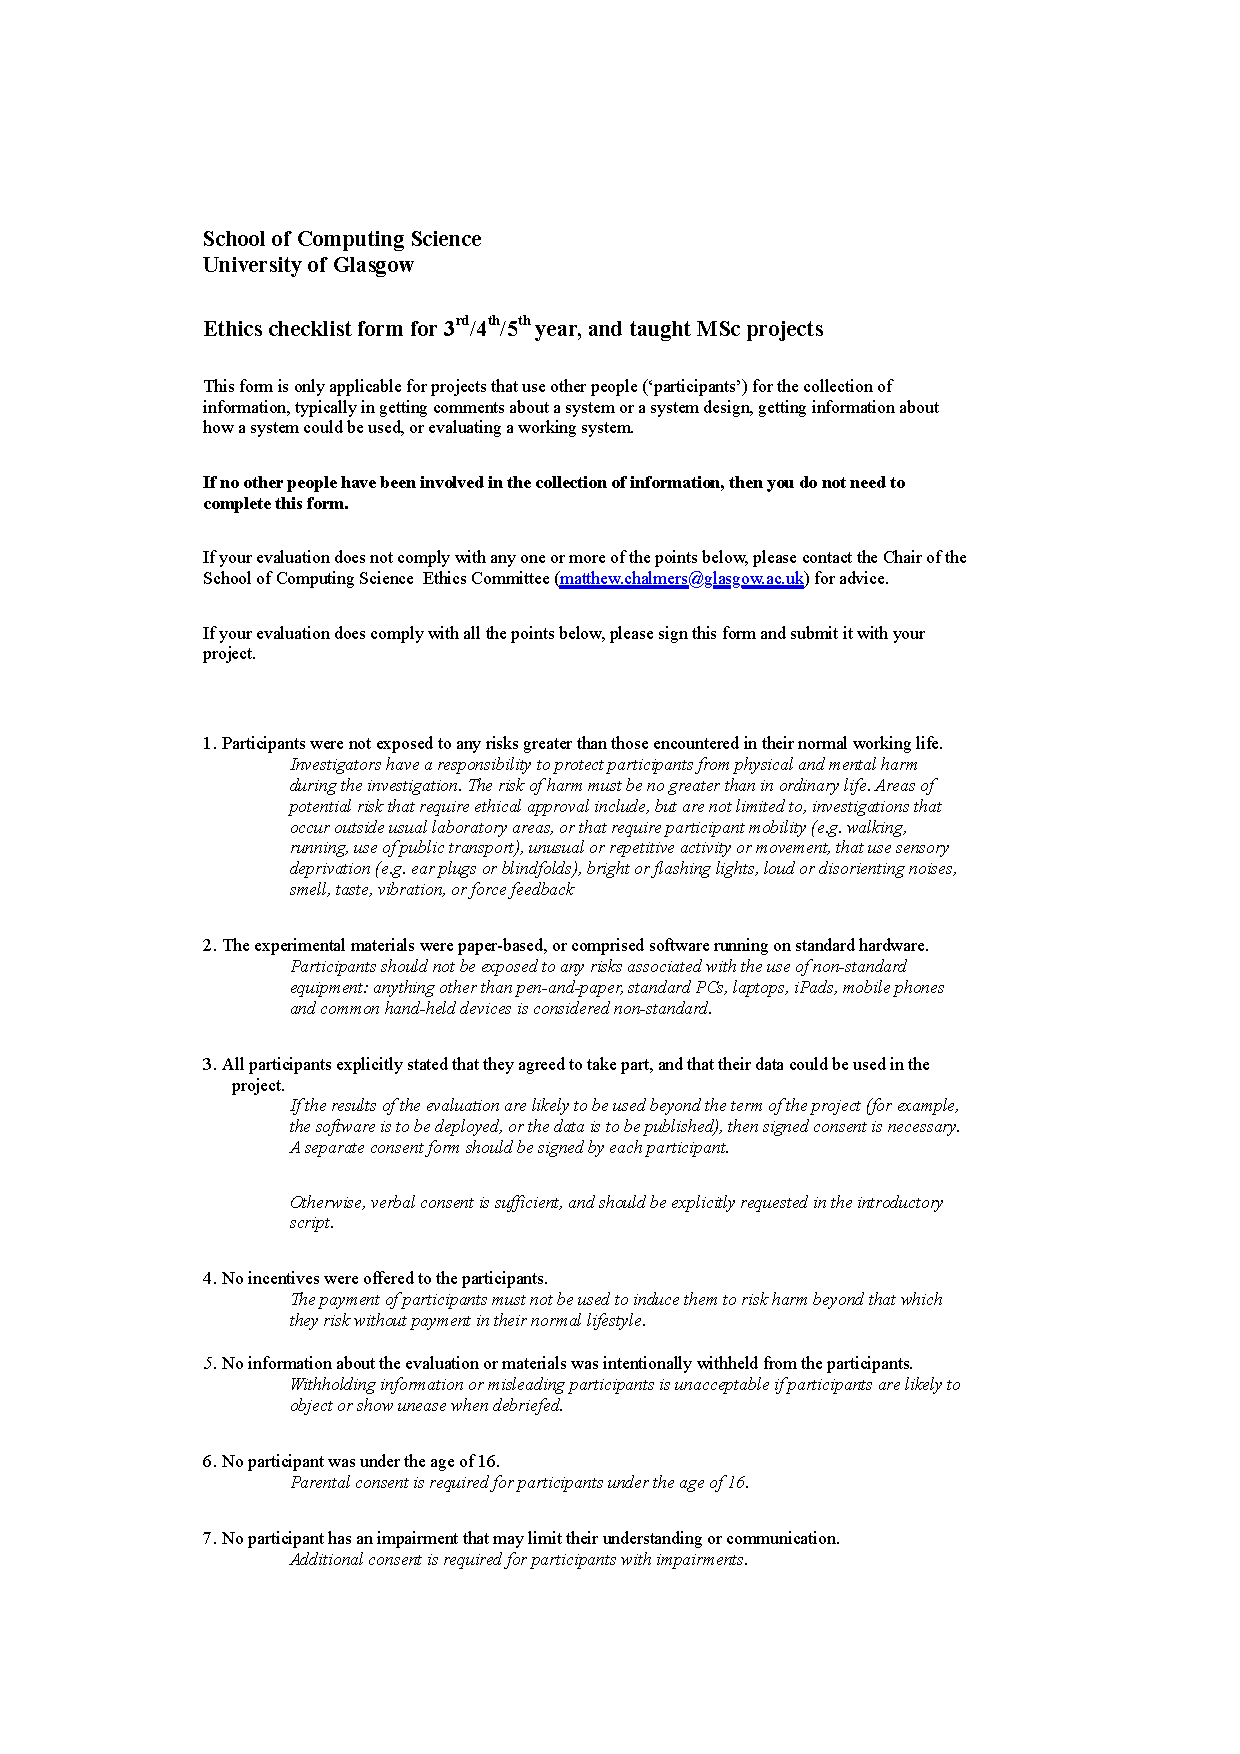
\includepdf[pages=-]{dissertation//images//myFigures//appendix//ethics.pdf}
     \label{ethics-checklist}
\section{Monitored user evaluation questions}
    
\includepdf[pages=-]{dissertation//images//myFigures//appendix//form.pdf}
     \label{survey-questions}
\section{Monitored user evaluation responses}
    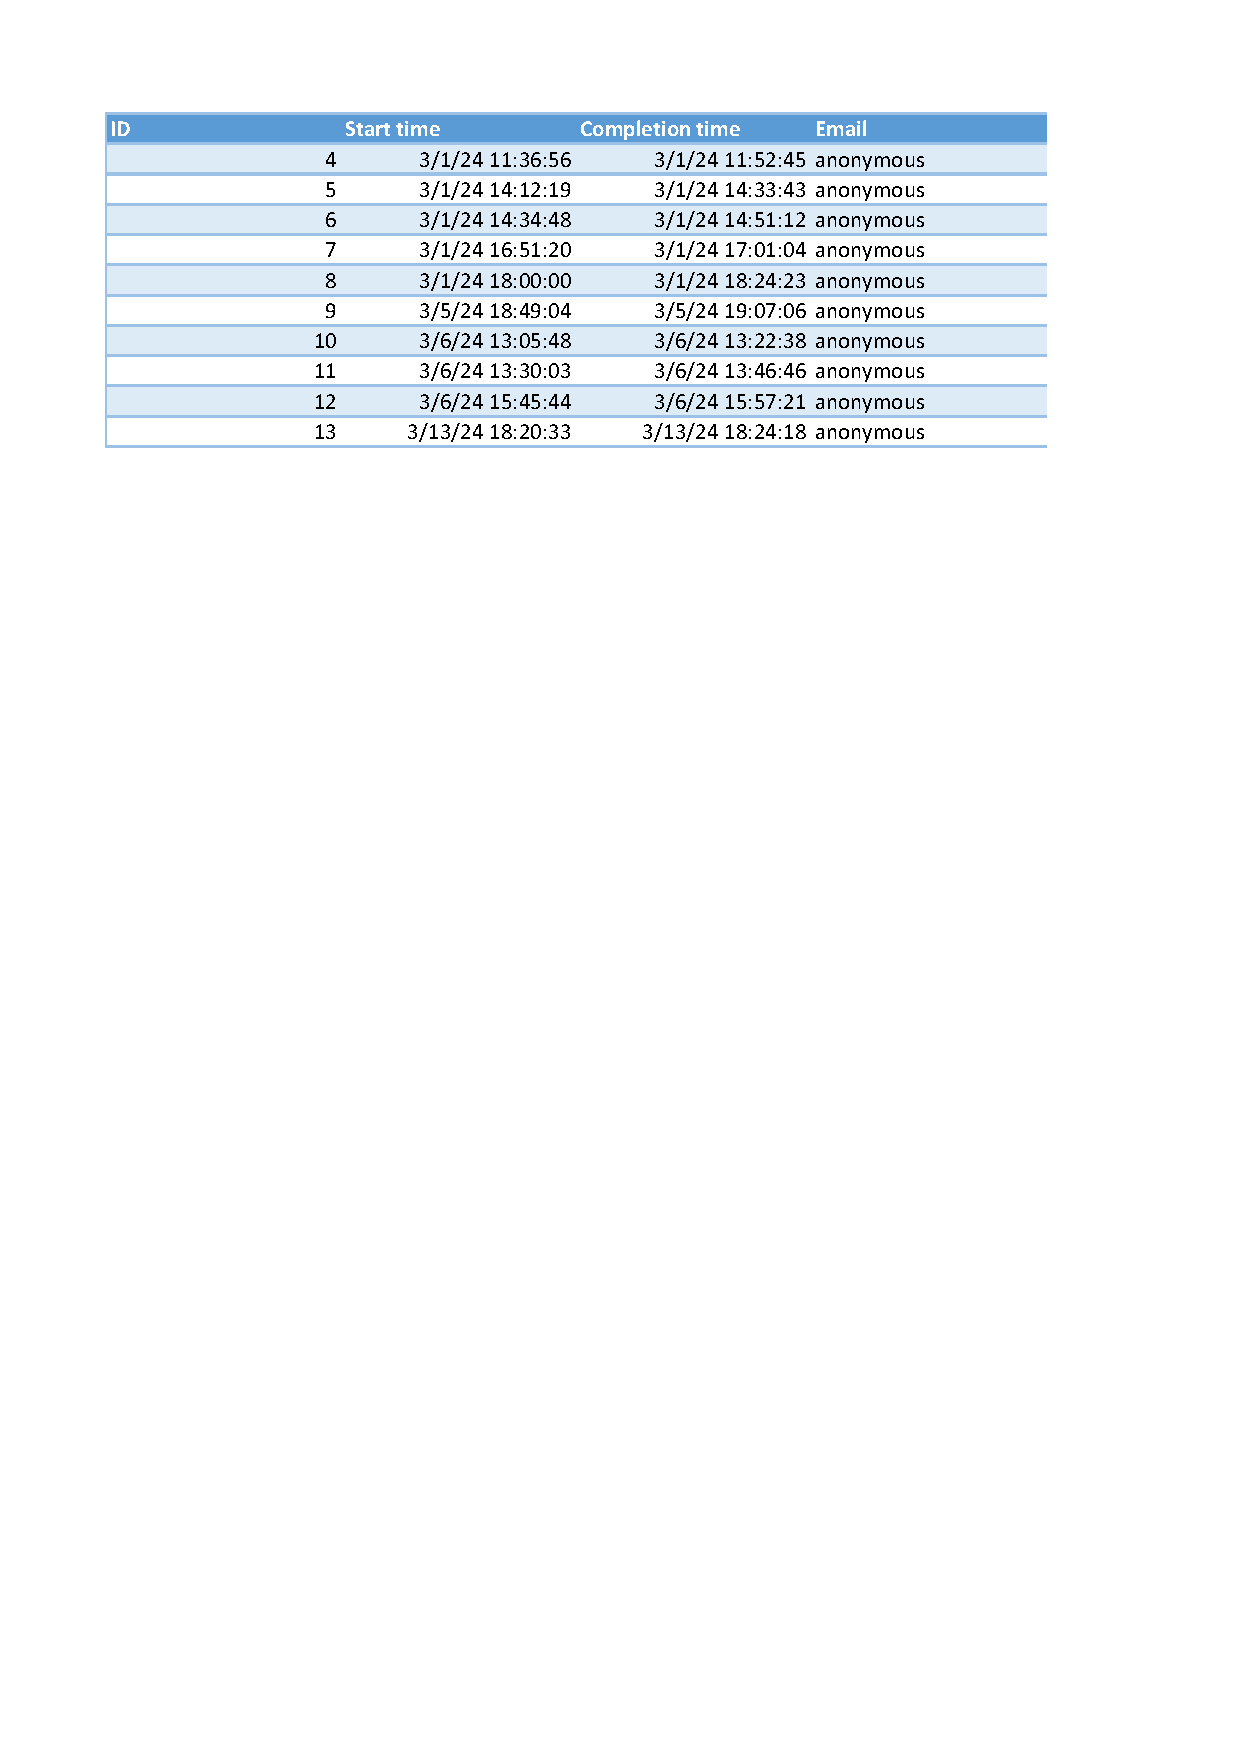
\includepdf[pages=-]{dissertation//images//myFigures//appendix//results.pdf}
     \label{fig:survey-results}
\section{Probability distributions text entry tooltip}
 \begin{figure} [H]
        \centering
        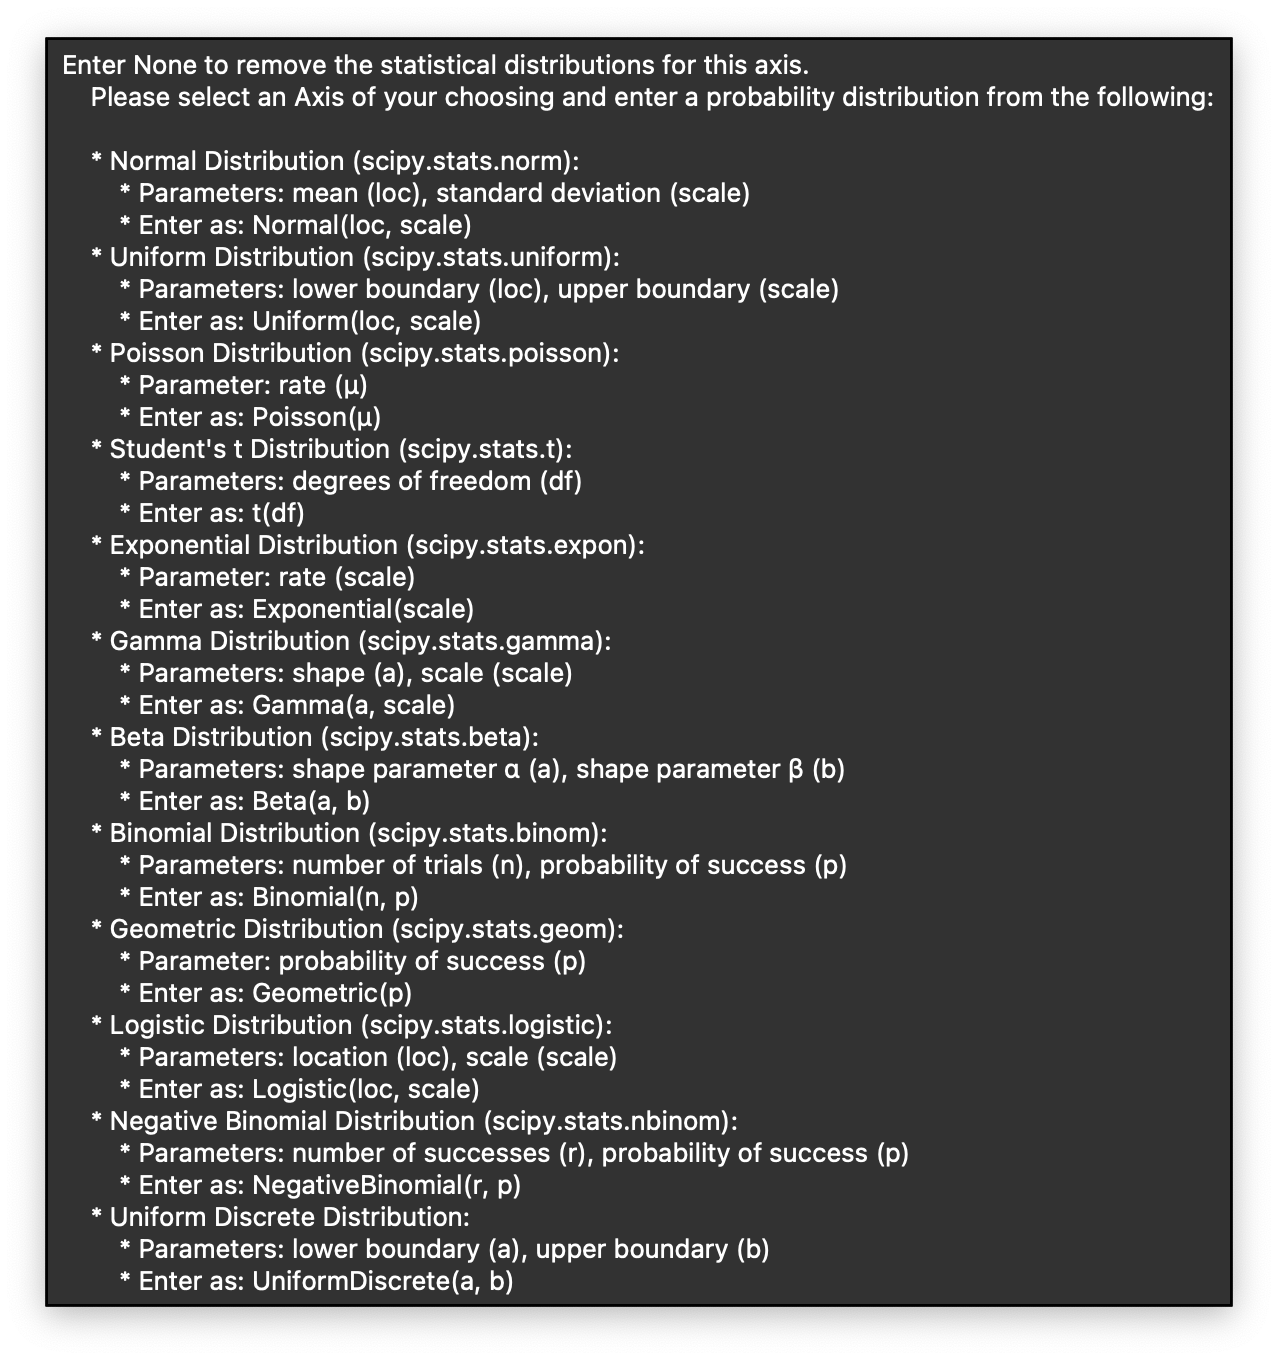
\includegraphics[width=1\linewidth]{dissertation//images//myFigures//appendix/prob.png}
        \caption{The tooltip showing all the probability distributions supported}
        \label{fig:prob-tooltip}
    \end{figure}
\section{BMI nomogram}
\begin{figure}[H]
        \centering
        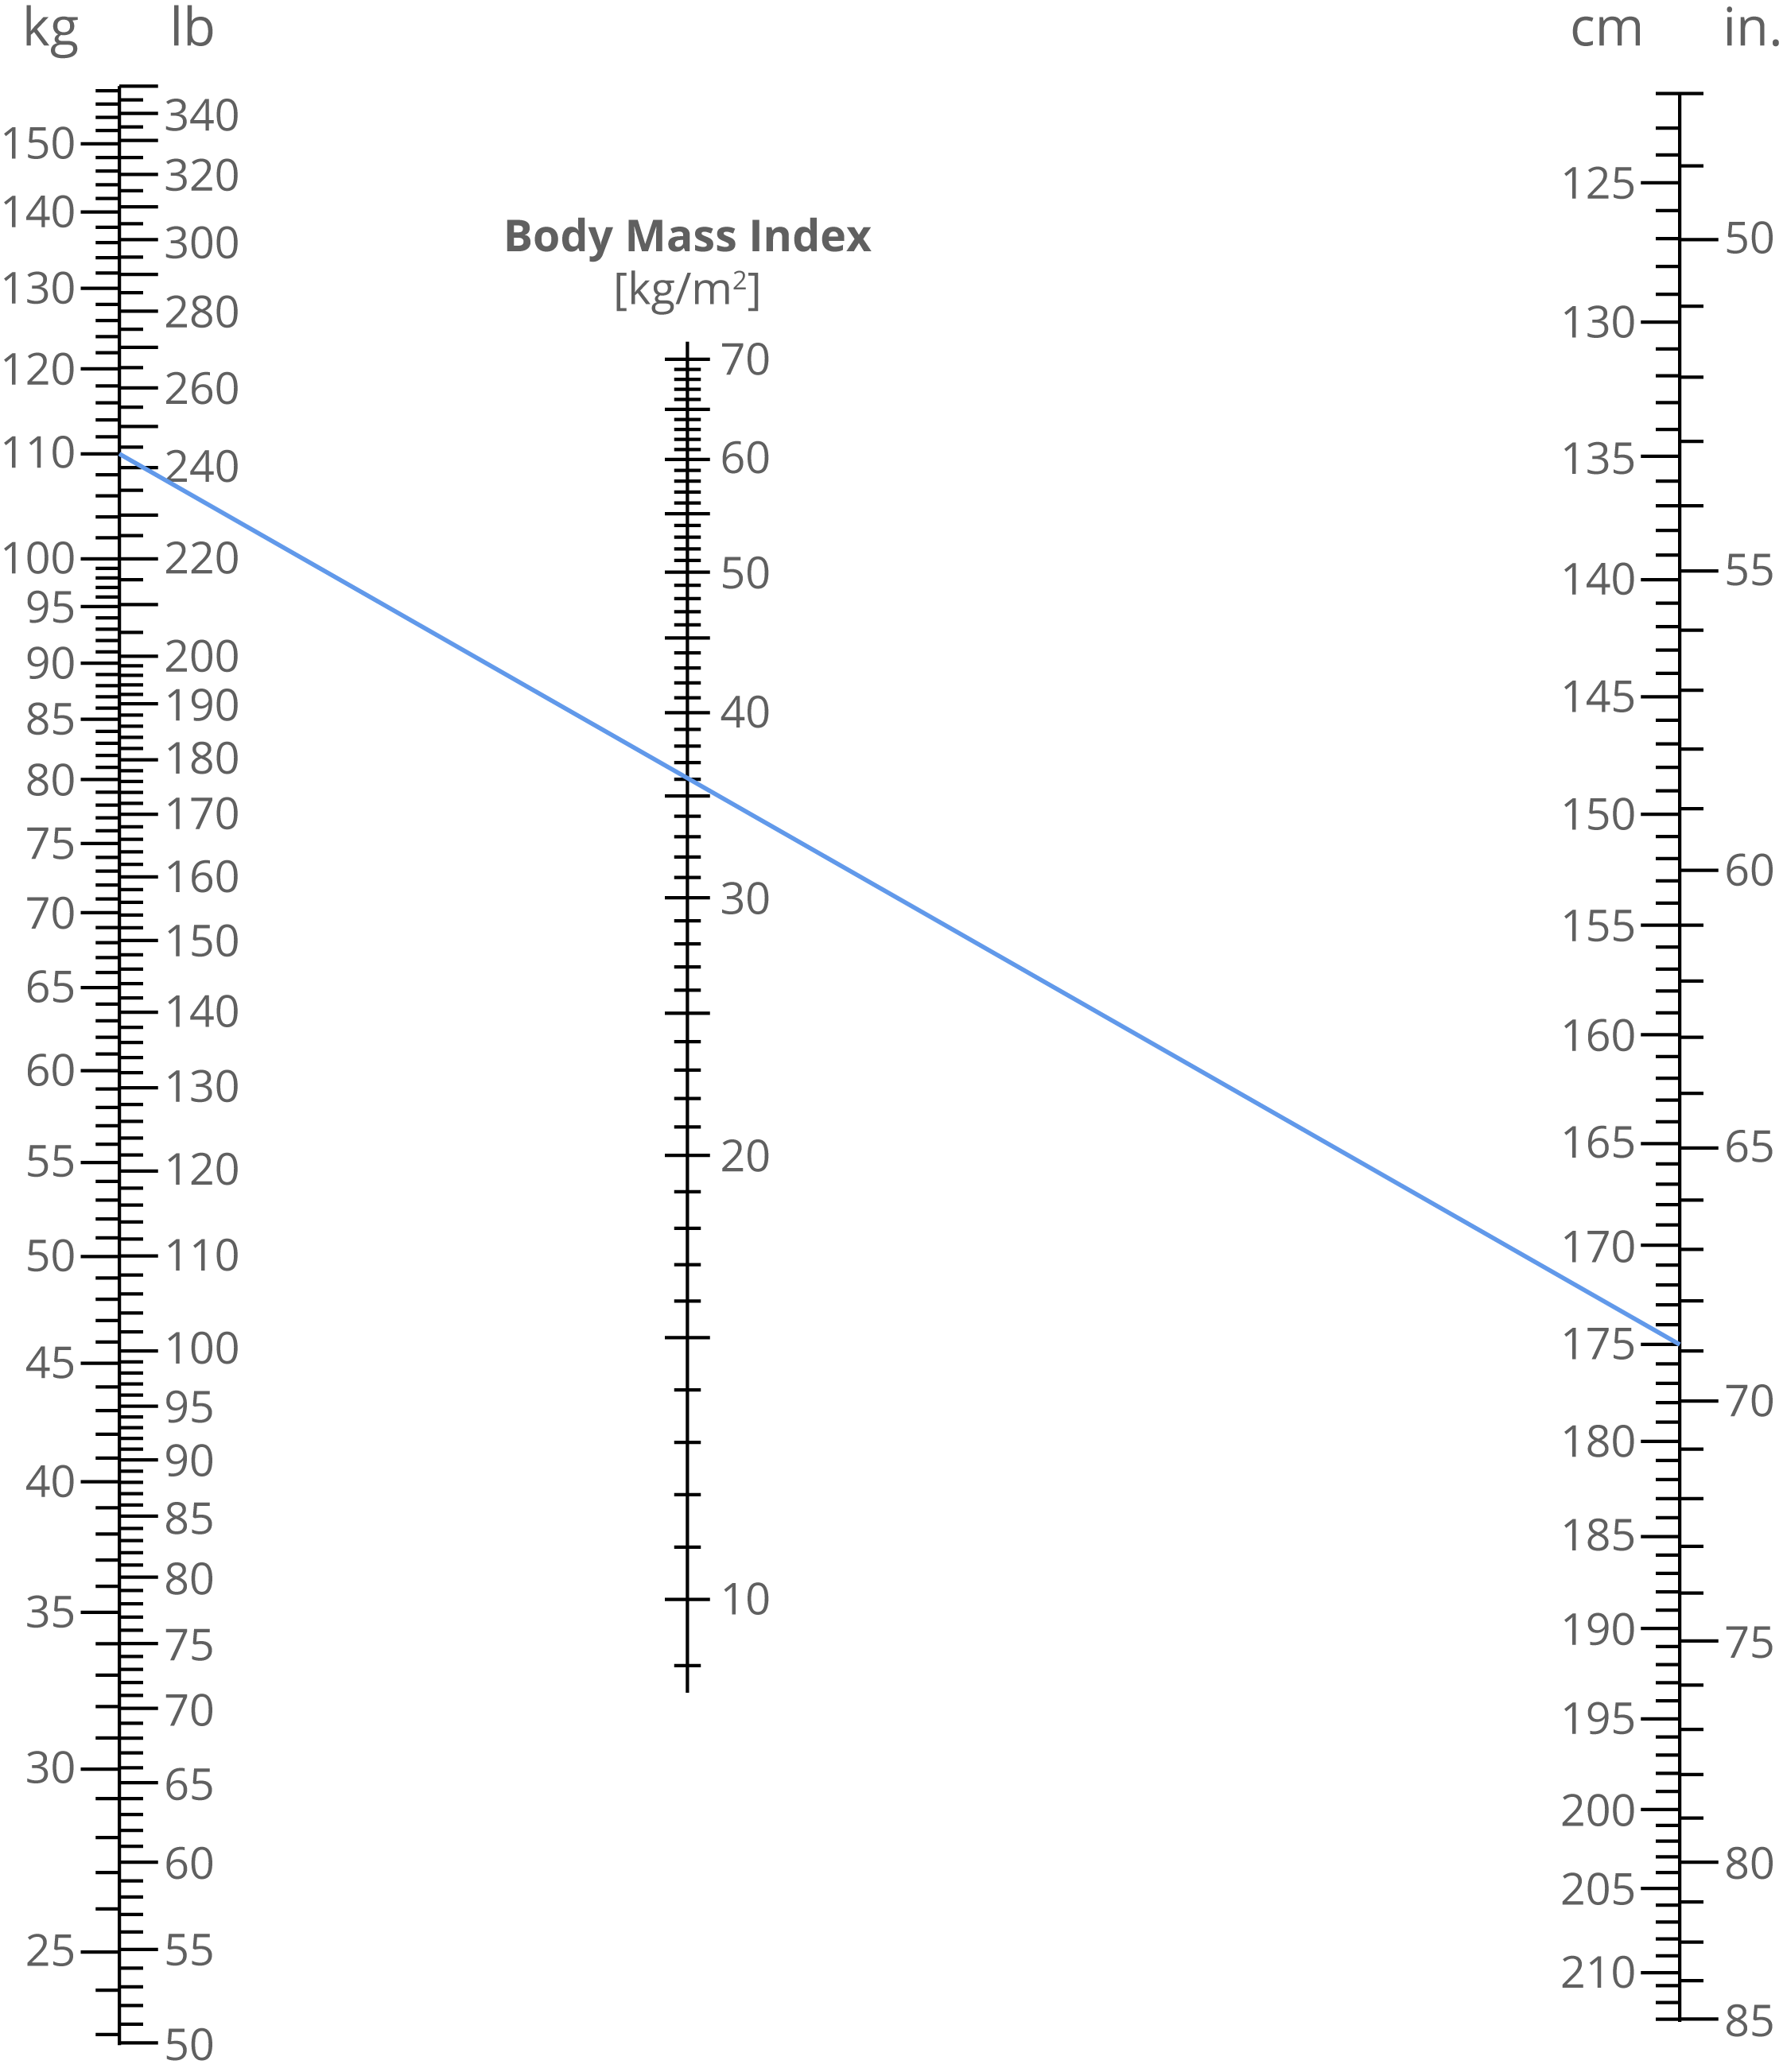
\includegraphics[width=1\linewidth]{dissertation//images//myFigures//appendix/bmi.png}
        \caption{The BMI nomogram \citep{merson-davies_body_2020}}
        \label{fig:bmi-nomogram}
    \end{figure}
\section{Fuel efficiency nomogram}
\begin{figure}[H]
        \centering
        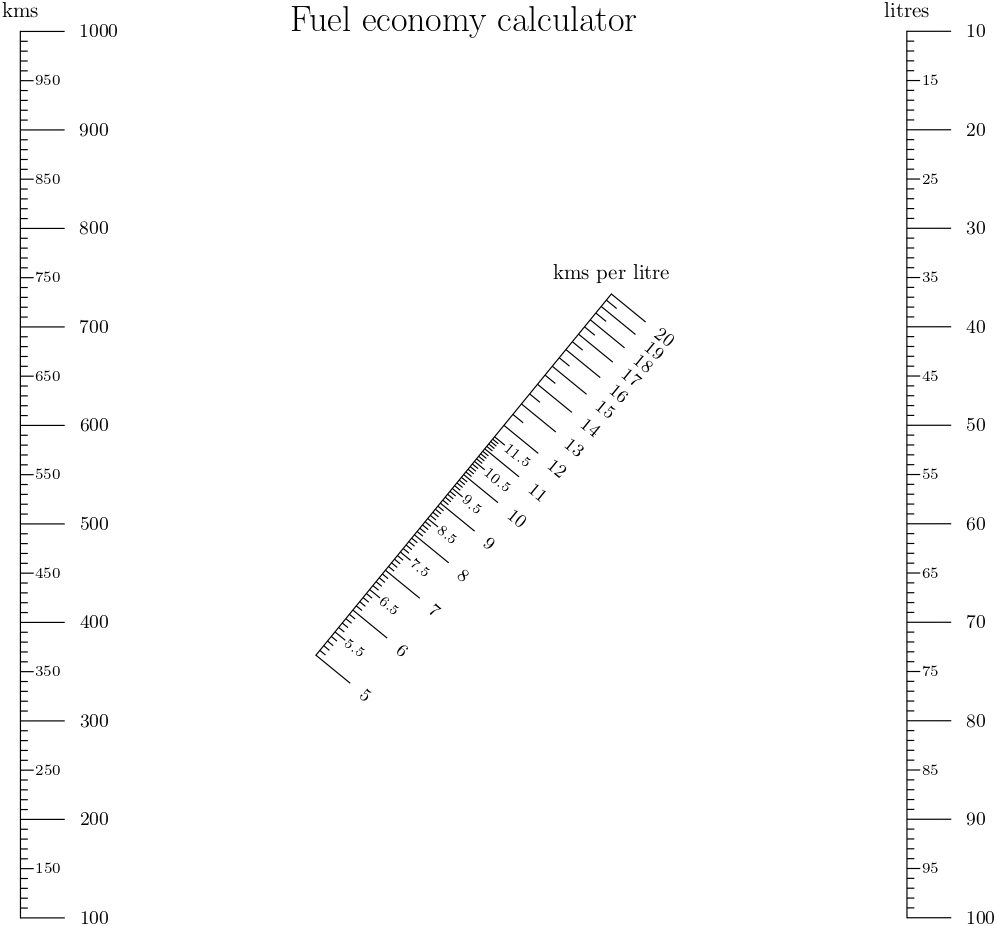
\includegraphics[width=1\linewidth]{dissertation//images//myFigures//appendix/fuel.jpg}
        \caption{The fuel efficiency nomogram \citep{boulet_PyNomo_2023}}
        \label{fig:fuel-efficiency}
    \end{figure}
\section{Slider crank mechanism nomogram}
\begin{figure}[H]
        \centering
        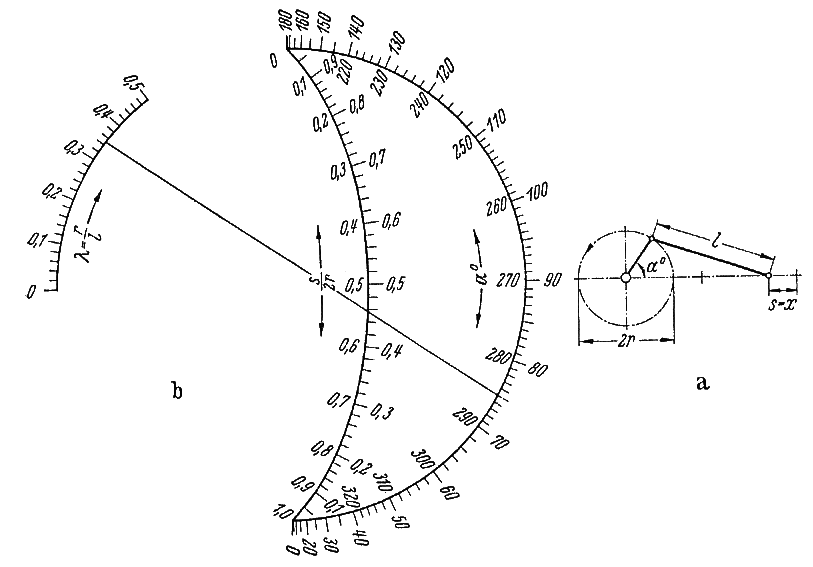
\includegraphics[width=1\linewidth]{dissertation//images//myFigures//appendix/meyer.png}
        \caption{The slider-crank mechanism nomogram \citep{boulet_PyNomo_2023}}
        \label{fig:slider-crank} 
    \end{figure}


\end{appendices}

%==================================================================================================================================
%   BIBLIOGRAPHY   

% The bibliography style is abbrvnat
% The bibliography always appears last, after the appendices.

\bibliographystyle{abbrvnat}

\bibliography{l4proj}

\end{document}
